\documentclass{article}
\usepackage{amsmath
                   ,siunitx
                   ,fancyhdr
                   ,amssymb
                   ,centernot
                   ,tikz
                   ,csquotes
                   ,graphicx
                   ,tocloft
                   ,titlesec
                   ,parskip
                   ,enumitem
                   ,hyperref}
\usepackage[margin=1in]{geometry}


%\renewcommand{\cftsecpresnum}{Lecture }  % Sets up the table of contents and section heading
\renewcommand{\cftdot}{.}
\renewcommand{\cftsecleader}{\cftdotfill{\cftdotsep}}
%\titlelabel{Lecture \thetitle}

\allowdisplaybreaks  % allows grouped equations like in align to go over the page
\graphicspath{ {./Images/} }  % tells graphicx where the images are stored relative to this file
\hypersetup{hidelinks}  % makes links invisible in table of contents
\setcounter{MaxMatrixCols}{20}

\renewcommand{\vec}[1]{\underline{#1}}
\renewcommand{\Re}{\operatorname{Re}}
\renewcommand{\Im}{\operatorname{Im}}
\newcommand{\cc}[1]{\overline{#1}}
\newcommand{\bb}[1]{\mathbb{#1}}
\newcommand{\A}{\,\forall\,}
\newcommand{\E}{\,\exists\,}
\newcommand{\hcf}{\operatorname{hcf}}
\newcommand{\lcm}{\operatorname{lcm}}
\newcommand{\sgn}{\operatorname{sgn}}
\newcommand{\binomeq}[2]{\frac{{#1}!}{{#2}!({#1}-{#2})!}}
\newcommand{\LUB}{\operatorname{LUB}}

\newcommand\mydiv[2]{%
$\strut#1$\kern.25em\smash{\raise.3ex\hbox{$\big)$}}$\mkern-8mu % This is used to do the division symbol like divisor)\overline{quotient} but nicer looking
      \overline{\enspace\strut#2}$}
      
\newcounter{example}[section]
\newenvironment{example}[1][]{\refstepcounter{example}\vspace{-0.2cm}
\subsubsection*{Example~\thesection.\theexample} \rmfamily}{\par}

% The stuff below makes the page layout not have stupidly huge margins and sets up header/footer
\pagestyle{fancy}
\lhead{Willoughby Seago}
\rhead{PPS Lecture notes}
\cfoot{Page \thepage}
\renewcommand{\headrulewidth}{0.4pt}
\renewcommand{\footrulewidth}{0.4pt}
\setlength{\parindent}{0pt}

% The stuff below is used for the title
\title{Proofs and Problem Solving Lecture Notes}
\author{Willoughby Seago}
\date{16 January 2019}

\newcommand{\notesVersion}{1.0}
\newcommand{\notesDate}{04/01/2021}

\begin{document}

\maketitle
These are my notes for the \textit{proofs and problem solving} course from the University of Edinburgh School of Mathematics, which I took as an optional course outside of the School of Physics.
When I took this course in the 2018/19 academic year it was taught by Dr Jonas Azzam\footnote{\url{https://www.maths.ed.ac.uk/school-of-mathematics/people/a-z?person=516}}.
These notes are based on the lectures delivered as part of this course, and the notes provided as part of this course, as well as the textbook for the course `A Concise Introduction to Pure Mathematics'\footnote{Liebeck, M \textit{A Concise Introduction To Pure Mathematics}, fourth edition (CRC Press, Boca Raton, 2016)}.
The content within is correct to the best of my knowledge but if you find a mistake or just disagree with something or think it could be improved please let me know.

These notes were produced using \LaTeX\footnote{\url{https://www.latex-project.org/}}.
Diagrams were drawn with tikz\footnote{\url{https://www.ctan.org/pkg/pgf}}.
Some images were taken from the lecture notes provided.

This is version \notesVersion~of these notes, which is up to date as of \notesDate.
\begin{flushright}
    Willoughby Seago
    
    s1824487@ed.ac.uk
\end{flushright}
\clearpage

\tableofcontents
\newpage
\section{Proofs}

\subsection*{What is a proof?}

A claim/proposition/theorem/lemma is an assertion that some statement follows from:

\begin{enumerate}
\item An assumption (eg. assuming that \(n\) is odd ...)
\item Some definition (eg. from the definition of integers ...)
\item Axioms (eg. the operations \(+,-,\cdot\))
\end{enumerate}

A proof is:

\begin{enumerate}
\item An explanation
\item Written in complete sentances
\item Comprehensible to any intelligent reader
\item Demonstrates how to deduce the claim
\end{enumerate}

A conjecture is a claim without proof but backed up by some evidence

\subsection*{Why are proofs so important?}

\begin{itemize}
\item Any falsehood propogates through any further mathematics
\item It isn't always obvious as to the validity of a claim
\item ``Obvious" statements are sometimes false
\item The proof can be more useful than the statement
\end{itemize}

\subsection*{Examples with \(\pi\)}

We define \(\pi\) as the area of the unit circle

\paragraph{Claim} The number \(\pi\) is also the ratio of a circles area \(A\) and the square of its radius \(r\). That is \(\pi=\frac{A}{r^2}\).

\paragraph{Proof} If \(T\) is a triangle and \(T'\) is a congruent triangle that is \(r\)-times the size of \(T\) then the area of \(T'\) is \(r^2\)-times the area of \(T\).

If \(S\) is the unit circle, write it as the union of triangles \(T_1,T_2,T_3,...\)

\begin{center}
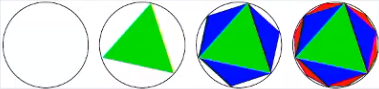
\includegraphics[scale=0.8]{CircleArea}
\end{center}

If we increase the size of \(S\) by a factor of \(r\) then we also increase the size of the triangles by a factor of \(r\). Therefore thee area of the triangles increases by a factor of \(r^2\) so the area of the circle increases by a factor of \(r^2\). Thus \(A=\pi r^2\implies \pi = \frac{A}{r^2}\). \(\blacksquare\)

Knowing that something exists is not the same as knowing it.

\paragraph{Claim} \(2\le\pi\le4\)

\paragraph{Proof} Consider the following unit circle with area \(\pi\) by definition and the two squares circumscribed and inscribed.

\begin{center}
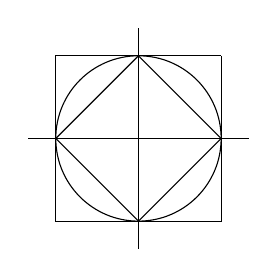
\begin{tikzpicture}[scale=0.7]
\draw (-2,0) -- (2,0);
\draw (0,-2) -- (0,2);
\draw (0,0) circle [radius=1.5];
\draw (-1.5,0) -- (0, 1.5) -- (1.5, 0) -- (0, -1.5) -- (-1.5, 0);
\draw (1.5, 1.5) -- (1.5, -1.5) -- (-1.5, -1.5) -- (-1.5, 1.5) -- (1.5, 1.5);
\end{tikzpicture}
\end{center}

The circumscribed square has an area larger than the area of the unit circle and the inscribed square has an area less than the area of the unit circle.

The circumscribed square has side length equal to two times the radius of the circle which means that it has side length 2 so area 4.

The inscribed square has diagonal equal to two times the radius of the circle which means that it has diagonal length 2 so by pythagoras the square has side length \(\sqrt 2\).

From the area of the three shapes and the knowledge of which is larger it follows that \(2\le\pi\le4\,\blacksquare\)

The following is an example of a bad (but technically correct) proof:

\paragraph{Claim} Every rational number is the sum of three cubes of rational numbers.

\paragraph{Proof} Let \(a\) be any rational number. Then a direct computation yields:
\[a=\left(\frac{a^3-3^5}{3^2a^2+3^4a+3^6}\right)^3+\left(\frac{-a^3+3^5a+3^6}{3^2a^2+3^4a+3^6}\right)^3+\left(\frac{a^2+3^4a}{3^2a^2+3^4a+3^6}\right)^3\,\blacksquare\]

This is a correct but not very good proof for a few reasons:
\begin{itemize}
\item It doesn't show the nature of the claim
\item It can't be repeated
\item It doesn't generalize
\item There exists a much better proof
\end{itemize}

Some plausible conjectors turn out to be false:

The prime number theorem:

\paragraph{Claim} If \(\pi(n)\) is the number of primes less than \(n\) and \(Li(n)=\int_0^n\frac{dx}{\log x}\), then:
\[\lim_{n\to\infty}\frac{\pi(n)}{Li(n)}\]
\begin{itemize}
\item Mathemeticians observed \(\pi(n)<Li(n)\) for many values of \(n\) (all values below \(10^{19}\) have been checked)
\item Gauss and Riesmann conjectured that \(\pi(n)<Li(n)\) for all \(n\)
\item But, Littlewood (1914) showed \(\pi(n)\ge Li(n)\) infinitley often.
\item All we know is that this first happens in the range \(n\in[10^{19},10^{317}]\)
\item For comparison there are only \(10^{80}\) protons in the universe
\end{itemize}

\section{Logic}

\subsection*{Logic}

If \(A\) and \(B\) are statements then:

\begin{itemize}
\item If \(A\) and \(B\) are statements then \(A\implies B\) means ``\(A\) implies \(B\)" or ``if \(A\) is true then \(B\) is true"
\item \(\bar A\) is the negation of statement \(A\)
\item If \(A\) is true then \(\bar A\) is false and vice versa
\item \(A\iff B\) means ``\(A\) and \(B\) are equivalent", that is \(A\implies B\) and \(B\implies A\). From this it follows that either \(A\) and \(B\) are true or \(A\) and \(B\) are false.
\item \(\bar{\bar{A}}\iff A\)
\item \(A\) or \(B\) means either \(A\) or \(B\) or both are true
\item \(A\) and \(B\) means \(A\) and \(B\) are both true
\item Statements about statements are allowed eg. \(\overline{(A \text{ and } B)}\iff(\bar A\text{ or } \bar B),\,\overline{(A \text{ or } B)}\iff(\bar A \text{ and } \bar B)\)
\end{itemize}

\[(A\implies B)\iff(\bar B\implies\bar A)\iff(\bar A \text{ or } B)\]
The above statements are equivalent to each other. (\(\bar B\implies \bar A\) is called the contrapositive of \(A\implies B\))

\paragraph{Claim} If \(A\) and \(B\) are statements then \((A\implies B)\iff(\bar B \implies \bar A)\)

\paragraph{Proof} Let us assume that \(A\implies B\). Then, if \(\bar B\) is true \(\bar A\) must also be true as if it were false then \(A\) would be true which implies \(B\) is true which it isn't. The same logic can be used when assuming the second statement and double negating to get the first statement. \(\blacksquare\)

The following is a proof by cases, every possible case is proved individualy which means that the statement is true. 

\paragraph{Claim} If \(A\) and \(B\) are statements then \((A\implies B)\iff(\bar A \text{ or } B)\).

\paragraph{Proof} We must show 1. if \(A\implies B\) then \(\bar A \text{ or } B\) is true and 2. if \(\bar A \text{ or } B\) is true then \(A\implies B\) is true.

\begin{enumerate}
\item Suppose \(A\implies B\) then we need to show that either \(\bar A\) or \(B\) is true. We do this by splitting into two further cases a. \(A\) is true and b. \(A\) is false.
\begin{enumerate}
\item \(A\) is true and since we have assumed that \(A\implies B\) it follows that \(B\) is true so \(\bar A\text{ or }B\) is true.
\item \(A\) is false so \(\bar A\) is true so \(\bar A\text{ or }B\) is true
\end{enumerate}
Since all cases give \(\bar A\text{ or }B\) is true given \(A\implies B\) it follows that \(\bar A\text{ or }B\) is true if\(A\implies B\)
\item Suppose \(\bar A\text{ or }B\) is true. We need to show \(A\implies B\) is true. Assume that \(A\) is true. Since we assume \(A\) is true \(\bar A\) must be false. Since we are also assuming \(\bar A\text{ or }B\) is true we must have \(B\) is true. Since \(B\) is true whenever \(A\) is true it follows that \(A\implies B.\)
\end{enumerate}
Since we have shown that \((A\implies B)\implies(\bar A \text{ or }B)\) and \((\bar A \text{ or }B)\implies(A\implies B)\) then \((A\implies B)\iff(\bar A \text{ or } B)\). \(\blacksquare\)

\paragraph{Claim} Let \(A\) and \(B\) be statements, then, \(\overline{(A\implies B)}\) is equivalent to \((A \text{ and } B)\).

\paragraph{Proof} By the previous claim \((A\implies B)\iff(\bar A \text{ or } B)\). Thus \(\overline{(A\implies B)}\iff\overline{(\bar A\text{ or }B)}\iff(\bar{\bar{A}}\text{ or } \bar B)\iff(A \text{ and } \bar B)\,\blacksquare\)

Proving \(A\implies B\) by contradiction means assuming \(overline{A\implies B}\) is true and showing that a logical contradiction occurs.

\paragraph{Claim} If \(m^2\) is even then \(m\) is even.

\paragraph{Proof} Assume \(m^2\) is even but \(m\) is odd. Then \(m=2n+1\) for some \(n\in\mathbb{Z}\). Hence \(m^2=(2n+1)^2=4n^2+4n+1=2(2n^2+2n)+1\) which is odd, but we assumed that \(m^2\) was even so this is a contradiction so \(m\) must be even. \(\blacksquare\)

\paragraph{Claim} Any false statement can imply anyother statement. That is if \(A\) and \(B\) are statements an \(A\) is false then \(A\implies B\)

\paragraph{Proof} Since \(A\) is false \(\bar A\) is true so \(\bar A \text{ or } B\) is true which is equivalent to \(A\implies B\,\blacksquare\)

\paragraph{corollary} If unicorns are real then \(1+1=3\)

\subsection*{Sets}

Sets are a collection of things called elements eg. \(\{1,2,3\}\) is the set of 1, 2 and 3.

Let \(S\) and \(T\) be two sets:

\begin{enumerate}
\item If \(S\) and \(T\) have the same elements then \(S=T\)
\item If \(x\) is an element of \(S\) then we write \(x\in S\)
\item If \(x\) is not an element of \(S\) then we write \(x\notin S\)
\item \(T\) is a subset of \(S\) if \((t\in T)\implies(t\in S)\)
\item If \(T\) is a subset of \(S\) we write \(T\subseteq S\)
\item If \(T\) is not a subset of \(S\) we write \(t\nsubseteq S\)
\item \(\{\}\) and \(\emptyset\) both represent the empty set (Nb \(\emptyset\) is a subset of all sets as there is no item in the empty set that isn't in any other set so it always follows the condition for subsets)
\end{enumerate}

\paragraph{Question} How many subsets does the set \(\{1,2,3\}\) have?

\paragraph{Answer}  It has 8 subsets:
\begin{itemize}
\item \(\{1,2,3\}\)
\item \(\{1,2\},\{1,3\},\{2,3\}\)
\item \(\{1\},\{2\},\{3\}\)
\item \(\emptyset\)
\end{itemize}

\section{Sets and Quantifiers}

Sets can be elements of other sets. For example \(S=\{a,b,\{c,d\}\}\) is the set containing elements \(a,b\) and \(\{c,d\}\)

There are different ways to denote a set. The following sets are all equivalent:

\begin{itemize}
\item The circle in \(\bb R^2\) with radius 1 and centre \((0,0)\)
\item The set of points \((x,y)\) in \(\bb R^2\) such that \(x^2+y^2=1\)
\item \(\{(x,y)\in\bb R^2|x^2+y^2=1\}\)
\end{itemize}

\subsection*{Quantifiers}

\begin{itemize}
\item \(\A\) means ``for all"
\item \(\E\) means ``there exists"
\item s.t. means ``such that"
\item \(!\) means negation \((!P\iff\bar P)\)
\end{itemize}

To negate a statement start by negating the entire statement and then move the \(!\) from left to right inverting quantifiers according to the following:

\begin{itemize}
\item \(!!P\iff P\)
\item \(!\A\longrightarrow\E!\)
\item \(!\E\longrightarrow\A!\)
\item \(=\longleftrightarrow\ne\)
\item \(\ge\longleftrightarrow<\)
\item \(\le\longleftrightarrow>\)
\item Negate the conclusion e.g \(!\)(\(x\) is odd)\(\longrightarrow x\) is even.
\end{itemize}

\begin{align*}
&!(\A n\in \bb Z,\E m\in\bb R\,st\,m^2=n)\\
\iff&\E n\in \bb Z,\,st\,!(\E m\in \bb R\,st\,m^2=n)\\
\iff&\E n\in \bb Z,\,st\,\A m\in \bb R\, !(m^2=n)\\
\iff&\E n\in \bb Z,\,st\,\A m\in \bb R\, m^2\ne n
\end{align*}

To prove a statement like \(\A x\in S,\,P(x)\) is true begin by letting \(x\) be any element in \(S\).

To prove a statement like \(\E x\in S,\,P(x)\) is true just find one \(x\) in \(S\) such that \(P(x)\) is true.

\paragraph{Claim} The statement ``\(A=\A n\in\bb Z\,\E m\in\bb R\,st\,m^2=n\)" is false

\paragraph{Proof} We will show that the negation is true. The negation is:
\[!A=\E n\in\bb Z\,st\,\A m\in\bb R, m^2\ne n\]
Let \(n=-1\). Now we will show that \(\A m\in\bb R m^2\ne-1\) which will prove \(!A\).

Let \(m\in\bb R\). Then \(m^2\ge 0>-1\implies m^2\ne-1\).

This proves \(!A\) is true so \(A\) is false. \(\blacksquare\)

\paragraph{Claim} \(\A n\in \bb Z\E m\in\bb Z\,st\,m>n\)

\paragraph{Proof} Let \(n\in Z\). We need to show that \(\E m\in\bb Z\,st\,m>n\).

Let \(m=n+1>n\) \(\blacksquare\)

\paragraph{Claim} \(\sqrt -\sqrt n\notin \bb Q\) for some \(n\in\bb Q\)

\paragraph{Proof} Proof by contradiction

Assume that \(\sqrt 2-\sqrt n\in \bb Q\)

By (3) we know that if \(a\in\bb Q,\,b\notin\bb Q\) then \(a+b\notin\bb Q\)

By (2) we know that if \(a,b\in\bb Q\) then \(a+b\in\bb Q\)

\[(\sqrt 2+\sqrt n)(\sqrt 2-\sqrt n)=2-n\]
By our initial assumption both \(\sqrt 2+\sqrt n\) and \(2-n\) are rational. Since \(ab\in\bb Q\) if both \(a\) and \(b\) are rational or both irrational this means that \(\sqrt 2-\sqrt n\) must be rational.
\[\sqrt 2-\sqrt n=-(\sqrt n-\sqrt 2)=\sqrt n+\sqrt 2-2\sqrt 2\]
From our initial assumption \(\sqrt n+\sqrt 2\) is rational and \(-2\sqrt2\) is irrational so it follows that \(\sqrt 2-\sqrt n\) is irrational. This is a contradiction so \(\sqrt 2+\sqrt n\notin\bb Q\) \(\blacksquare\)

\paragraph{Claim} \(\A a,b\in\bb R\) if \(a<b\) then \(\E r\in\bb Q\,st\,a<r<b\)

\paragraph{Proof} Let \(n\) be such that \(\frac1n<b-a\implies n>\frac{1}{b-a}\)

Let \(j\) be the largest integers such that \(\frac jn\le a\)

Since \(j\) is the maximum \(\frac{j+1}{n}>a\)

\(\frac{j+1}{n}=\frac jn+\frac1n<\frac jn+b-a\le a+b-a=b\)

Thus \(a<\frac{j+1}{n}<b\) and \(\frac{j+1}{n}\in\bb Q\) \(\blacksquare\)

\section{Decimals}

\subsection*{Geometric series}

For \(x\in\bb R\):
\[\sum_{n=1}^k x^k=x+x^2+\dotsb+x^k=\frac{x-x^{k+1}}{1-x}\]
For \(|x|<1\):
\[\sum_{n=1}^\infty x^k=x+x^2+x^3+\dotsb=\frac{x}{1-x}\]
For \(|x|>1\)
\[\sum_{n=1}^\infty (\frac 1x)^k=\frac{1}{x}+\frac{1}{x^2}+\frac{1}{x^3}+\dotsb=\frac{\frac 1x}{1-\frac 1x}=\frac{1}{x-1}\]

\paragraph{Claim} \(0.\overline{12}=\frac{4}{33}\)

\paragraph{Proof} We will write \(0.\bar{12}\) as a geometric series

\begin{align*}
0.\overline{12}&=\frac{1}{10}+\frac{2}{10^2}+\frac{1}{10^3}+\frac{2}{10^4}+\dotsb\\
&=\frac{10}{10^2}+\frac{2}{10^2}+\frac{10}{10^4}+\frac{2}{10^4}+\dotsb\\
&=\frac{12}{10^2}+\frac{12}{10^4}+\dotsb\\
&=12\left(\frac{1}{10^2}+\frac{1}{10^4}+\dotsb\right)\\
&=12\left(\frac{1}{10^2}+\left(\frac{1}{10^2}\right)^2+\dotsb\right)\\
&=12\left(\frac{1}{10^2-1}\right)\\
&=\frac{4}{33}\quad\blacksquare
\end{align*}

A decimal can be written as \(a_0.a_1a_2a_3\dotso\) where \(a_n\in\bb Z\) and \(0\le a_n\le9\). There is only one way to represent most numbers unless they end with a string on 9s:
\[a_0.a_1a_2\dotso a_{k-1}a_k9\dotso9\equiv a_0.a_1a_2\dotso a_{k-1}(a_k+1)0\dotso0\]
Formaly two numbers \(a_0.a_1a_2\dotso\) and \(b_0.b_1b_2\dotso\) are equal if and only if there exists \(k\in N\) such that:
\begin{itemize}
\item For \(j<k\) we have \(a_j=b_j\)
\item For \(j=k\) we have \(a_j=b_j+1\)
\item For \(j>k\) we have \(a_j=0,\,b_j=9\)
\end{itemize}

\paragraph{Claim} Every real number \(x\in\bb R\) has a decimal expansion \(x=a_0.a_1a_2\dotso\)

\paragraph{Proof} Let \(x\in\bb R\)

Pick \(a_0\in\bb Z\) such that \(a_0\le x<a_0+1\)

Pick \(a_0\in\bb Z\) such that \(a_0+\frac{a_1}{10}\le x<a_0+\frac{a_1+1}{10}\)

\(0\le a_0<10\), if \(a_1\ge10\) then \(a_0+1\le a_0+\frac{a_1}{10}\le x<a_0+1\) which is a contradiction so \(0\le a_0<10\).

Continue for \(a_n\). As \(n\to\infty\), \(|x-a_0.a_1a_2\dotso a_n|=0\) so \(x=a_0.a_1a_2\dotso\quad\blacksquare\)


\subsection*{Pigeon hole principle}

Suppose \(k>n\) and we have \(a_1,\dotsc,a_k\in S\) with \(|S|=n\). Then there exists \(i\ne j\) such that \(a_i=a_j\) 

\paragraph{Claim} \(\frac 17\) has a repeating decimal

\paragraph{Proof} Using the division algorithm:

\begin{center}
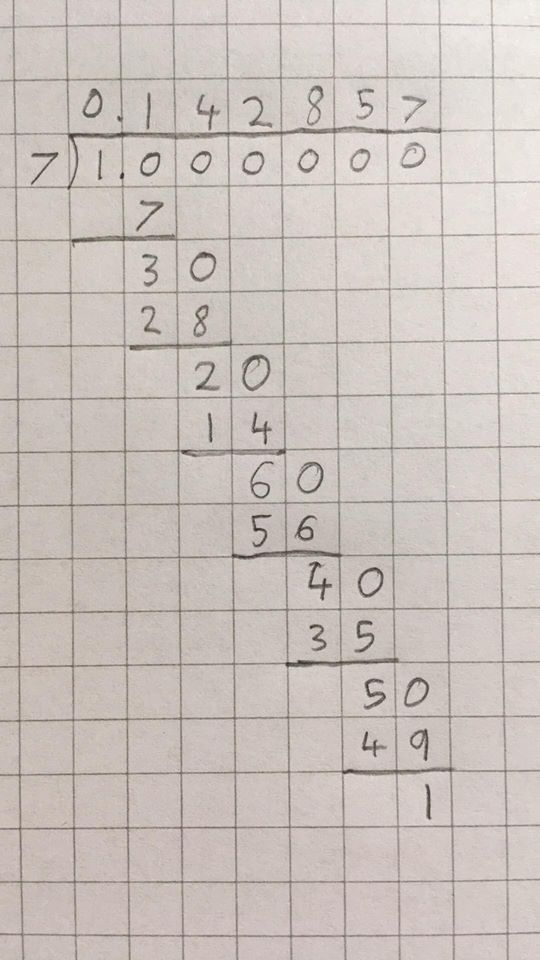
\includegraphics[scale=0.3, trim= 0.6cm 4.6cm 3cm 2.8cm, clip]{1dividedby7}
\end{center}

The remainder is again one which will result in a repeat of the expansion from the last time the remainder was one. This shows that \(\frac 17=0.\overline{142857}\) which is a repeating decimal.\(\quad\blacksquare\)

\paragraph{Claim} A real number \(x\in\bb R\) has a periodic decimal expansion \(\iff x\in\bb Q\)

\paragraph{Proof} We need to prove the implication both ways:
\begin{itemize}
\item A real number \(x\in\bb R\) has a periodic decimal expansion \(\implies x\in\bb Q\):

Let \(x=a_0.a_1a_2\dotso a_k\overline{b_1\dotso b_l}\)
Let \(a=a_1a_2\dotso a_k\) and \(b=b_1\dotso b_l\)
Then:
\[x=a_0+\frac{a}{10^k}+\frac{1}{10^k}\cdot\frac{b}{10^l-1}\]
Therefore \(x\) has a periodic decimal expansion.

\item \(x\in\bb Q\implies\)A real number \(x\in\bb R\) has a periodic decimal expansion:

Each step of the long division algorithm \mydiv{q}{p.000\dotso} returns a remainder in \(1,\dotsc,q\). By the pigeon hole princile ome remainder \(k\) must occur twice. Because \(p.000\dotso\) has trailing zeroes the algorithm repeats at that point. The period of \(\frac pq\) is at most \(q-1\).
\end{itemize}
The implication is true in both directions so the claim is true.\(\quad\blacksquare\)

All of this works in different bases:

For \(n>1\) we say \(x\) has base \(n\) expansion
\[b_jb_{j-1}\dotso b_0.a_1a_2a_3\dotso\]
For integers \(b_i,a_i\in\{0,1,2,\dotsc,n\}\) if
\[x=n^jb_j+n^{j-1}b_{j-1}+\dotsb+nb_1+b_0+\frac{a_1}{n}+\frac{a_2}{n^2}+\frac{a_3}{n^3}\dotsb\]

\begin{example}
If \(x=0.\overline{012}\) in base 3 find \(x\) as a fraction in base 10

\begin{align*}
x&=0+\frac{0}{3}+\frac{1}{3^2}+\frac{2}{3^3}+\frac{0}{3^4}+\frac{1}{3^5}+\frac{2}{3^6}+\dotsb\\
&=\frac{3\cdot0+1\cdot3^2+2\cdot3^3}{3^3}+\frac{3\cdot0+1\cdot3^2+2\cdot3^3}{3^6}+\dotsb\\
&=\frac{5}{3^3}+\frac{5}{3^6}+\dotsb\\
&=5\left(\frac{1}{3^3}+\frac{1}{3^6}\right)\\
&=5\left(\frac{1}{3^3}+\left(\frac{1}{3^3}\right)^2\right)\\
&=5\cdot\frac{1}{3^3-1}\\
&=\frac{5}{26}
\end{align*}
\end{example}
\section{Inequalities}

\subsection*{Defining \(</>\)}

Given \(x,y\in\bb R\) we may write \(x<y\) which we pronounce ``\(x\) is less than \(y\)" or \(y>x\) which we pronounce ``\(y\) is greater than \(x\)". The symbols \(<\) and \(>\) satisfy the the following axioms:
\begin{enumerate}
\item Positive/negative - If \(x\in\bb R\) then exactly one of the following is true:
\begin{itemize}
\item \(x<0\)
\item \(x=0\)
\item \(x>0\)
\end{itemize}
\item Negations reverse - If \(x>y\) then \(-x<-y\)
\item Adding constants - If \(x>y\) and \(c\in\bb R\) then \(x+c>y+c\)
\item Positive multiplication - If \(x>0\) and \(y>0\) then \(xy>0\)
\item Transitive property - If \(x>y\) and, for \(z\in\bb R\), \(y>z\) then \(x>z\)
\end{enumerate}
This is a minimum set of axioms. No axiom can be deduced from the others.

This captures the essence of ``\(</>\)" but we must prove some things.

All apart from the first axiom apply to \(\le/\ge\)

\paragraph{Claim} For any \(x,y\in\bb R\) exactly one of the following is true: \(x>y,\,x=y\text{ or }x<y\)
\paragraph{Proof} Let \(x,y\in\bb R\). By axiom 1 exactly one of the following is true:
\[x-y>0,\quad x-y=0\quad\text{ or }\quad x-y<0\]
By axiom 3 with \(c=y\)
\[ x-y+y>0+y,\quad x-y+y=0+y\quad\text{ or }\quad x-y+y<0+y\]
Simplifying:
\[x>y,\quad x=y\quad\text{ or }\quad x<y\quad\blacksquare\]

\paragraph{Claim} \(\sqrt{xy}\le\frac{x+y}{2}\)
\paragraph{Proof} By Liebeck example 5.2
\begin{align*}
&0\le(a-b)^2\\
\implies&0\le a^2+b^2-2ab\\
\intertext{By axiom 3 with \(c=2ab\)}
\implies&2ab\le a^2+b^2\quad(5.1)\\
\intertext{By axiom 4 if \(u>v>0\) and \(c>0\) then \(cu>cv\), applying this to (5.1) with \(c=\frac 12\)}
\implies&ab\le\frac{a^2+b^2}{2}\\
\intertext{Let \(a=\sqrt x\) and \(b=\sqrt y\)}
\implies&\sqrt x \sqrt y\le\frac{\sqrt x^2\sqrt y^2}{2}\\
\implies&\sqrt{xy}\le\frac{x+y}{2}\quad\blacksquare
\end{align*}

\paragraph{Claim} If \(x>y>0\) then \(\frac 1x<\frac 1y\)

\paragraph{Proof} We will prove the contrapositve:

For \(x,y>0\) if \(\frac 1x\ge\frac 1y\) then \(x\le y\)

Suppose that \(\frac 1x\ge\frac 1y\). By axiom 4:
\begin{align*}
&\frac 1x\ge\frac 1y\\
\implies&x\cdot\frac 1x\ge x\cdot\frac 1y\\
\implies&1\ge\frac xy\\
\implies&y\cdot1\ge y\cdot\frac xy\\
\implies &y\ge x\\
\implies&x\le y\quad \blacksquare
\end{align*}

\paragraph{Claim} Let \(u,v>0\) then \(u>v\iff u^2>v^2\)

\paragraph{Proof} Suppose that \(u,v>0\).

We need to prove the implication in both directions:
\begin{itemize}
\item \(u>v\implies u^2>v^2\)

Assume \(u>v\) we need to show \(u^2>v^2\). By axiom 3:
\begin{align*}
&u>v\\
\implies&u-v>v-v\\
\implies&u-v>0\\
\intertext{Since \(u,v>0\) by axiom 3:}
\implies&u>0\\
\implies&u+v>0+v\\
\implies&u+v>v>0\\
\intertext{Since \(u+v>0\) and \(u-v>0\) then by axiom4:}
\implies&(u+v)(u-v)>0\\
\implies&u^2-v^2>0\\
\implies&u^2>v^2
\end{align*}
\item \(u^2>v^2\implies u>v\)
Take the contrapositive:
\[u\le v\implies u>v\]
Then since we didn't use axiom 1 by the same process as above but with \(\le\) instead of \(>\) we get \(u^2>v^2\implies u>v\)
\end{itemize}
We have proved the implication in both directions so the claim is true. \(\blacksquare\)

\section{Exponentiation}

\paragraph{Claim} For \(u,v,x\in\bb R,\,x>0\) if \(u>v\) then \(xu>xv\)

\paragraph{Proof} Let \(u>v\) and \(x>0\) for all \(u,v,x\in\bb R\)

By axiom 3 with \(c=-v\):
\[u>v\implies u-v>v-v=0\]
By axiom 4:
\[x(u-v)>0\implies xu-xv>0\]
By axiom 3 with \(c=xv\): 
\[xu-xv>0\implies xu-xv+xv>xv\implies xu>xv\quad \blacksquare\]

\subsection*{Roots}

\paragraph{Proposition} \(\A x>0\) and \(n\in\bb N\,\E\) a unique number \(y>0\) such thant \(y^n=x\).

We denote this number as \(y=x^{\frac 1n}\).

For \(m,n\in\bb N\) if \(m,n>0\) then we define \(x^{\frac mn}=(x^m)^{\frac 1n}\)

\paragraph{Claim} If \(x>0\) and \(\frac mn\in\bb Q\) then \(x^{\frac mn}=(x^m)^{\frac 1n}\)

\paragraph{Proof} Since the number \(y>0\) such that \(y^n=x^m\) is unique \(\left(\text{and equal to } (x^m)^{\frac 1n}\right)\) then we just need to show that \(\left(x^{\frac mn}\right)^n=x^m\).
\[\left(x^{\frac mn}\right)^n=\left(\left(x^{\frac 1n}\right)^m\right)^n=\left(x^{\frac 1n}\right)^{mn}=\left(\left(x^{\frac 1n}\right)^n\right)^m=\left(x^{\frac nn}\right)^m=x^m\quad\blacksquare\]

\paragraph{Claim} If \(x>0\) and \(m,n\in\bb N\) then \(\left(x^{\frac 1n}\right)^{\frac 1m}=x^{\frac{1}{mn}}\)

\paragraph{Proof} Since the \((mn)^{\text{th}}\) root is unique we just need to show that \(\left[\left(x^{\frac 1n}\right)^{\frac 1m}\right]^{mn}=x\):
\[\left[\left(x^{\frac 1n}\right)^{\frac 1m}\right]^{mn}=\left[\left(\left(x^{\frac 1n}\right)^{\frac 1m}\right)^m\right]^n=\left[x^{\frac 1n}\right]^n=x\quad\blacksquare\]

\paragraph{Claim} \(100^{10000}>10000^{100}\)

\paragraph{Proof} \[100=10^2,\quad10000=10^4\]
\[100^{10000}=(10^2)^{10000}=10^{20000}\]
\[10000^{100}=(10^4)^{100}=10^{400}\]
Since both bases are the same and \(20000>400\) then \(100^{10000}>10000^{100}\quad\blacksquare\)

\paragraph{Claim} \(\sqrt[3]{3}>\sqrt 2\)

\paragraph{Proof} -
\begin{align*}
&\sqrt[3]{3}>\sqrt 2\\
\iff&3^{\frac 13}>2^{\frac 12}\\
\intertext{By Liebeck example 5.4:}
\iff&\left(3^{\frac 13}\right)^2>\left(2^{\frac 12}\right)^2\\
\iff&3^{\frac 23}>2\\
\intertext{By homework 2 problem 4:}
\iff&\left(3^{\frac 23}\right)^3>2^3\\
\iff&3^2>2^3\\
\iff&9>8
\end{align*}
Since this is true and the implication goes both ways then \(\sqrt[3]2>\sqrt 2\quad\blacksquare\)

\paragraph{Claim} For \(x_1,x_2,y_1,y_2\in\bb R\):
\[x_1y_1+x_2y_2\le\sqrt{x_1^2+x_2^2}\cdot\sqrt{y_1^2+y_2^2}\]

\paragraph{Proof} Assume \(x_1,x_2,y_1,y_2>0\) as if they are negative then the LHS would be smaller without the RHS decreasing.

Assume \(\sqrt{x_1^2+x_2^2}=\sqrt{y_1^2+y_2^2}=1\)
Recall from previous proof that \(ab\le \frac{a^2+b^2}{2}\). Hence:
\[x_1y_1+x_2y_2\le\frac{x_1^2+y_1^2}{2}+\frac{x_2^2+y_2^2}{2}=\frac{x_1^2+x_2^2}{2}+\frac{y_1^2+y_2^2}{2}\]
Since \(\sqrt{x_1^2+x_2^2}=\sqrt{y_1^2+y_2^2}=1\) then \(x_1^2+x_2^2=y_1^2+y_2^2=1\):
\[x_1y_1+x_2y_2\le\frac 12+\frac 12=1=1\cdot1=\sqrt{x_1^2+x_2^2}\cdot\sqrt{y_1^2+y_2^2}\]
Now for the general case assume that \(x_1,x_2,y_1,y_2\in\bb R\) and let:
\[a_1=\frac{x_1}{\sqrt{x_1^2+x_2^2}}\quad\&\quad a_2=\frac{x_2}{\sqrt{x_1^2+x_2^2}}\]
\[b_1=\frac{y_1}{\sqrt{y_1^2+y_2^2}}\quad\&\quad b_2=\frac{y_2}{\sqrt{y_1^2+y_2^2}}\]
\[\sqrt{a_1^2+a_2^2}=\left[\frac{x_1^2}{x_1^2+x_2^2}+\frac{x_2^2}{x_1^2+x_2^2}\right]^{\frac 12}=\left[\frac{x_1^2+x_2^2}{x_1^2+x_2^2}\right]^{\frac 12}=[1]^{\frac 12}=1\]
By the same logic \(\sqrt{b_1^2+b_2^2}=1\)
So by applying the previous case we get:
\[1\ge a_1b_1+a_2b_2=\frac{x_1}{\sqrt{x_1^2+x_2^2}}\cdot\frac{y_1}{\sqrt{y_1^2+y_2^2}}+\frac{x_2}{\sqrt{x_1^2+x_2^2}}\cdot\frac{y_2}{\sqrt{y_1^2+y_2^2}}\]
\[1\ge \frac{x_1y_1}{\sqrt{x_1^2+x_2^2}\cdot\sqrt{y_1^2+y_2^2}}+\frac{x_2y_2}{\sqrt{x_1^2+x_2^2}\cdot\sqrt{y_1^2+y_2^2}}\]
\[1\ge \frac{x_1y_1+x_2y_2}{\sqrt{x_1^2+x_2^2}\cdot\sqrt{y_1^2+y_2^2}}\]
\[\frac{1}{x_1y_1+x_2y_2}\ge \frac{1}{\sqrt{x_1^2+x_2^2}\cdot\sqrt{y_1^2+y_2^2}}\]
By a previous proof if \(x\ge y>0\) then \(\frac 1y\ge\frac 1x\):
\[x_1y_1+x_2y_2\le\sqrt{x_1^2+x_2^2}\cdot\sqrt{y_1^2+y_2^2}\quad\blacksquare\]

\section{Complex Numbers}

A number \(z\) is in the set of complex numbers \(\bb C\) if \(z=x+iy,\,x,y\in\bb R,\,i^2=-1\).

\begin{center}
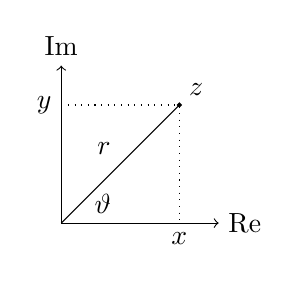
\begin{tikzpicture}
\draw [<->] (2,0) -- (0,0) -- (0,2);
\node [right] at (2,0) {Re};
\node [above] at (0,2) {Im};
\draw (0,0) -- (1.5,1.5);
\draw [dotted] (0,1.5) -- (1.5,1.5) -- (1.5,0);
\node [above right] at (1.5,1.5) {\(z\)};
\node [above left] at (0.75,0.75) {\(r\)};
\draw [fill] (1.5,1.5) circle [radius=0.025];
\node [below] at (1.5,0) {\(x\)};
\node [left] at (0,1.5) {\(y\)};
\node [above right] at (0.3,0) {\(\vartheta\)};
\end{tikzpicture}
\end{center}

\[x=\Re(z),\quad y=\Im(z),\quad\vartheta=\arg(z)\quad\&\quad r=|z|=\sqrt{x^2+y^2}\]
\[z=x+iy=r(\cos\vartheta+i\sin\vartheta)=re^{i\vartheta}\]
The complex conjugate of \(z\) is denoted \(\bar z\) It is a reflection in the real axis. \(\bar z=x-iy\)
\[\bar z=x-iy=r(\cos\vartheta-i\sin\vartheta)=r(\cos(-\vartheta)+i\sin(-\vartheta))=re^{-i\vartheta}\]

If \(z=re^{i\vartheta}\) and \(w=se^{i\varphi}\) then \(zw\) is given by:
\[zw=rse^{i(\vartheta+\varphi)}\]
From this we can see:
\[|zw|=|z||w|\quad\&\quad\arg(zw)=\arg(z)+\arg(w)\]

\section{More Complex Numbers}

\begin{example}
What is the locus of points such that \(\frac 12=|z-1-i|\)?

\(|z|\) is the distance from the origin to \(z\).

\(|z-w|\) is the distance from \(z\) to \(w\).

Let \(z=x+yi\) for some \(x,y\in\bb R\)
\[|z-1-i|=|x+yi-1-i|=|(x-1)+(y-1)i|=\sqrt{(x-1)^2+(y-1)^2}=\frac 12\]
This is a circle center \(1+i\) radius \(\frac 12\)
\end{example}
\begin{example}
What is the locus of points such that \(|z-1|=|z+1|\)?

Using the fact that \(|w|^2=w\bar w\):
\[|z-1|^2=|z+1|^2\]
\[\implies (z-1)\overline{(z+1)}=(z+1)\overline{(z+1)}\]
Using the fact that \(\overline{(a+b)}=\bar a +\bar b\):
\[\implies (z-1)(\bar z-1)=(z+1)(\bar z+1)\]
\[\implies z\bar z -z-\bar z+1=z\bar z+z+\bar z+1\]
\[\implies -z-\bar z=z\bar z\]
\[\implies 0=2(z+\bar z)\]
Using the fact that \(z+\bar z=2\Re(z)\):
\[\implies 0=2(2\Re(z))\]
\[\implies \Re(z)=0\]
So the set of points is given by:
\[\{z:|z-1|=|z+1|\}=\text{Imaginary axis}=\{yi:y\in\bb R\}\]
\end{example}
\subsection*{Roots of unity}

We want to find solutions to \(z^n=1\). One obvious solution is \(z=1\). The funamental theorem of algebra tells us that a degree \(n\) polynomial has \(n\) roots (including multiplicity). If we let \(w\) be another root to the equation then:
\[w^n=1\implies w^n=\left(e^{\frac{2\pi i}{n}}\right)^n=e^{2\pi i}=\cos 2\pi+i\sin 2\pi=1+0i=1\]

\paragraph{Claim} \(1,w,w^2,\dotsc,w^{n-1}\) are \(n\) distinct solutions to the equation \(z^n=1\)

\paragraph{Proof} First we will prove that they are solutions:

Let \(j\in\bb R\) such that \(0\le j\le n-1\) and \(w\) be a root such that \(w^n=1\):
\[\left(w^j\right)^n=w^{jn}=\left(w^n\right)^j=1^j=1\]
So \(w^j\) is  a root.

Now we must show that they are distinct solutions, we will do this by contradiction:

Let \(j,k\in\bb R\) such that \(0\le j<k\le n-1\)

Assume that \(w^j=w^k\)
\[\implies 1=w^{j-k}=\left(e^{\frac{2\pi i}{n}}\right)^{j-k}=e^{\frac{2\pi(j-k)i}{n}}=\cos\frac{\frac{2\pi(j-k)i}{n}}+i\sin{\frac{2\pi(j-k)i}{n}}=1\]
This only happens when \(\frac{2\pi (j-k)i}{n}\) is an integer multiple of \(2\pi\)
\[\implies \frac{j-k}{n}\in\bb Z\]
This is not posible as \(0\le j<k\le n-1\implies 0\le k-j<n\) thus \(w^j\ne w^k\) so the roots are distinct\(\quad\blacksquare\)

\begin{example}
Find the solutions to \(z^2=1\)
\[e^{\frac{2\pi i}{2}}=e^{\pi i}=-1\]
Also 1 is an obvious root as \(1^2=1\)
\end{example}
\paragraph{Claim} If one solution to \(z^n=p\) for some \(p\in\bb C\) is \(z=q\) then the roots are given by \(q,wq,w^2q,\dotsc,w^{n-1}q\) where \(w=e^{\frac{2\pi i}{n}}\)

\paragraph{Proof} \(\left(w^jq\right)^n=w^{jn}q^n=1p=p\) Since \(w,w^2,\dotsc,w^{n-1}\) are distinct then \(q,wq,w^2q,\dotsc,w^{n-1}q\) are distinct.\(\quad\blacksquare\)

\begin{example}
Find the solutions to \(z^2=-1\). \(z=i\) is an obvious solution. The second roots of unity are 1 and -1 so the solutions are \(i\) and \(-i\)
\end{example}
\section{Polynomials}

An \(n\)-degree polynomial has the form:
\[p(z)=a_nz^n+a_{n-1}z^{n-1}+\dotsb+a_1z+a_0\]
Where \(a_n\ne0\) and \(a_i\in\bb c\,\A i\). We say that \(\alpha\) is a root of \(p(z)\) if \(p(\alpha)=0\). A complex polynomial has coefficients in \(\bb C\), a real polynomial only has coefficients (but not necesserily roots) in \(\bb R\). Any complex polynomial has at least one root in \(\bb C\). If \(\alpha\) is a root of \(p(z)\) then we can write \(p(z)=(z-\alpha)q(z)\) where \(q(z)\) is another polynomial. Repeated application of this shows that all polynomials can be factored into the product of linear terms:
\[p(z)=a(z-r)(z-r_2)\dotsm(z-r_n)\]
Where \(r_i\) is a root such that \(p(r_i)=0\,\A i\). Some roots may repeat. If a root occurs \(m\) times in \(r_1,r_2,\dotsc,r_n\) then we say it has multiplicity \(m\).

\paragraph{Claim} If \(p\) is a real polynomial and \(r\) is a root then \(\cc r\) is a root.

\paragraph{Proof} If \(p(x)=a_0+a_1x+\dotsb+a_nx^n\) with \(a_i\in\bb R\) and \(p(r)=0\) then:
\begin{align*}
0&=p(r)\\
&=\cc{p(r)}\qquad(\text{Using the fact that if \(c\in\bb R\) then \(\cc c=c\)})\\
&=\cc{a_0+a_1r+\dotsb+a_nr^n}\\
&=\cc{a_0}+\cc{a_1r}+\dotsb+\cc{a_nr^n}\qquad(\text{Using the fact that \(\cc{z+w}=\cc z+\cc w\)})\\
&=\cc{a_0}+\cc{a_1}\bar r+\dotsb+\cc{a_n}\cc{r^n}\qquad(\text{Using the fact that \(\cc{zw}=\bar z\cc w\)})\\
&=a_0+a_1\cc r+\dotsb+a_n\cc{r^n}\\
&=a_0+a_1\cc r+\dotsb+a_n(\cc r)^n\qquad(\text{Repeated application of \(\cc{zw}=\bar z\cc w\)})\\
&=p(\cc r)
\end{align*}
So \(p(\cc r)=0\) so \(\cc r\) is a root\(\quad\blacksquare\)

If \(p(z)=z^n+a_{n-1}z^{n-1}+\dotsb+a_1z+a_0\) has roots \(r_1,r_2,\dotsc,r_n\) then:
\[r_1+r_2+\dotsb+r_n=\sum_ir_i=-a_{n-1}\]
\[r_1r_2\dotsm r_n=\prod_ir_i=(-1)^na_0\]

\paragraph{Claim} If \(p\) and \(q\) are \(n\) degree polynomials and they share \(n+1\) distinct roots then \(p=q\).

\paragraph{Proof} Let \(h=p-q\) then \(h\) is a degree \(n\) polynomial with \(n+1\) distinct roots \(x_1,x_2,\dotsc,x_{n+1}\) by Liebeck theorem 7.2 we know:
\[h(x)=a(x-x_1)(x-x_2)\dotsm(x-x_n)\]
Since they are distinct we know that \(x_{n+1}\ne x_i\) for \(i=1,2,\dotsc,n\). We also know that by Liebeck theorem 7.2:
\[0=h(x_{n+1})=a(x_{n+1}-x_1)(x_{n+1}-x_2)\dotsm(x_{n+1}-x_n)\]
None of the linear terms can be zero so \(a=0\) which means that \(h=0\) that is \(p-q=0\) and this can only happen if \(p=q\quad\blacksquare\)

\section{Induction}

\subsection*{Summation notation}

\[\sum_{k=m}^n=a_m+a_{m+1}+\dotsb+a_n\]
It is possible to do a change of variables:
\[\sum_{k=m}^na_{k+p}=a_{m+p}+a_{m+p+1}+\dotsb+a_{n+p}=\sum_{k=m+p}^{n+p}a_k\]

\subsection*{Product notation}

\[\prod_{k=m}^na_k=a_ka_{k+1}\dotsm a_n\]

\subsection*{Induction}

Let \(k\) be a known integer

Let \(P(n)\) be a statement that makes sense for any integer \(n\ge k\).

The principle of induction is then:
\begin{itemize}
\item \(P(k)\) is true
\item \(P(n)\implies P(n+1)\) for any integer \(n\ge k\)
\end{itemize}
Then my mathematical induction \(P(n)\) is true for all integers \(n\ge k\).

\paragraph{Claim} \(n^3+2n\) is divisible by 3 for all integers \(n\ge 1\)

\paragraph{Proof} We will use proof by induction

Let \(P(n)\) be the statement ``\(n^3+2n\) is divisible by 3".

\emph{Base case:}

If \(n=1\) then \(n^3+2n=1^3+2(1)=3\) which is divisible by 3

\emph{Induction step:}

Assume \(P(n)\) is true for some integer \(n\ge 1\)

We will show \(P(n+1)\) is true:

\begin{align*}
&(n+1)^3+2(n+1)\\
=&n^3+3n^2+3n+1+2n+2\\
=&n^3+2n+3n^2+3n+3\\
=&\underbrace{n^3+2n}_{\text{divisible by 3 by assumption}}+\underbrace{3(n^2+n+1)}_{\text{divisible by 3 as has factor of 3}}\\
\implies&(n+1)^3+2(n+1)\text{ is divisible by 3}=P(n+1)
\end{align*}
So \(P(n)\implies P(n+1)\) and the base case is true so the claim is true\(\quad\blacksquare\)

Not all statements naturally start at \(n=1\)

For which \(n\) do we have \(2^n>n+3\)?

Let \(P(n)\) be the statement ``\(2^n>n+3\)"
\begin{align*}
n=1:\quad&2^1<1+3\implies P(1)\text{ is false}\\
n=2:\quad&2^2<2+3\implies P(2)\text{ is false}\\
n=3:\quad&2^3>3+3\implies P(3)\text{ is true}\\
n=4:\quad&2^4>4+3\implies P(4)\text{ is true}
\end{align*}
It looks like \(P(n)\) is true for integers \(n\ge 3\)

\paragraph{Claim} \(2^n>n+3\,\A n\ge 3\)

\paragraph{Proof} We will use proof by induction

Let \(P(n)\) be the claim ``\(2^n>n+3\)"
 
\emph{Base case:}

\(P(3)\iff2^3>3+3\iff8>6\) this is true so \(P(3)\) is true

\emph{Induction step:}

Assume \(P(n)\) is true

We want to show \(2^{n+1}>n+1+3=n+4\)

\[2^{n+1}=2\cdot2^n>2(n+3)=2n+6>n+4\]

So \(P(n)\implies P(n+1)\) and thebase case is true so the by induction the claim is true\(\quad\blacksquare\)

The union of two sets is a new set that contains all of the elements that are in at least one of the two sets. The union of sets \(A\) and \(B\) is written \(A\cup B\). The intersection of two sets is a new set that contains all of the elements that are found in both of the sets. The intersection of sets \(A\) and \(B\) is written \(A\cap B\)

\paragraph{Claim} A set of size \(n\) has \(2^n\) subsets \(\A n\ge0\)

\paragraph{Proof} We will use proof by induction

Let \(P(n)\) be the statement ``A set of size \(n\) has \(2^n\) subsets"

\emph{Base case:}

When \(n=0\) the set is \(\emptyset\) which has one subset (\(\emptyset\subseteq T\,\A T\) by definition). \(2^n=2^0=1\) so \(P(0)\) is true.

\emph{Induction step:}

Assume that \(P(n)\) is true for some \(n\ge0\)

We will show \(P(n+1)\)

Let \(S\) be a set with \(n+1\) elements.

Let \(a\in S\) and \(A=\{x\in S|x\ne a\}\) (That is \(A\) is the set \(S\) with element \(a\) removed). From this it can be seen that \(A\subseteq S\) and \(|A|=|S|-1=n+1-1=n\).

There are two cases for subsets of \(S\):
\begin{enumerate}
\item Case 1 Let \(E\) be a set such that \(E\subseteq A\) this implies that \(E\subseteq S\). There are by assumption \(2^n\) subsets of \(A\).
\item Case 2 Every subset of \(S\) that is not a subset of \(A\) must contain \(a\) thus everyone of these subsets is of the form \(E\cup\{a\}=\{x\in E\text{ or }x=a\}\) so by the assumption there are \(2^n\) such sets.
\end{enumerate}
These two cases encompass all subsets of \(S\) so \(S\) has \(2^n+2^n=2\cdot 2^n=2^{n+1}\) subsets so \(P(n+1)\) is true if \(P(n\) is true so by induction \(P(n)\) is true \(\A n\ge0\)

\section{Strong induction}

Given a convex polyhedron with \(n\) vertices how many diagonals does it have?

\begin{center}
\begin{tabular}{|c|c|c|}\hline
\(n\) & Shape & Number of diagonals\\ \hline
3 & Triangle & 0\\
4 & Quadrilateral & 2\\
5 & Pentagon & 5\\
6 & Hexagon & 9\\ \hline
\end{tabular}
\end{center}

Let \(f(n)\) be the number of diagonals that a convex \(n\)-gon has.

\begin{center}
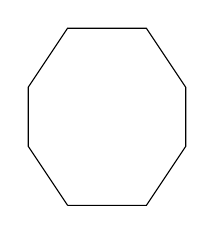
\begin{tikzpicture}[scale=0.5]
\draw (0,0) -- (2,0) -- (3,1.5) -- (3,3) -- (2,4.5) -- (0,4.5) -- (-1,3) -- (-1,1.5) -- (0,0);
\end{tikzpicture}
\end{center}

This is shape \(P\) it is a convex \(n\)-gon. From \(P\) we construct a new shape by adding an edge between two vertices:

\begin{center}
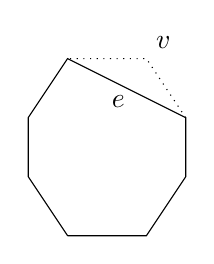
\begin{tikzpicture}[scale=0.5]
\draw (0,0) -- (2,0) -- (3,1.5) -- (3,3) -- (0,4.5) -- (-1,3) -- (-1,1.5) -- (0,0);
\draw [dotted] (3,3) -- (2,4.5) -- (0,4.5);
\node [above right] at (2,4.5) {\(v\)};
\node [below left] at (1.7,3.8) {\(e\)};
\end{tikzpicture}
\end{center}

This is shape \(P'\) it is a convex \((n-1)\)-gon. \(P'\) has \(f(n-1\) diagonals. \(P\) has the following diagonals that \(P'\) doesn't:
\begin{enumerate}
\item \(n-3\) diagonals from \(v\) (\(v\) can't make diagonals with its self or with its direct neighbours)
\item The diagonal where \(e\) is
\end{enumerate}

Thus \(P\) has 
\[f(n)=\underbrace{f(n-1)}_{\text{From }P'}+\underbrace{n-3}_{\text{From (1)}}+\underbrace{1}_{\text{from (2)}}=f(n-1)+n-2\]

From this it is possible to work out \(f(n)\) as a sum:
\begin{align*}
f(n)&=f(n-1)+n-2\\
&=f(n-2)+n-3+n-2\\
&=f(n-3)+n-4+n-3+n-2\\
&\,\,\,\vdots\\
&=\underbrace{f(3)}_{=0}+2+3+\dotsb+n-2\\
&=\sum_{k=2}^{n-2}k
\end{align*}

\paragraph{Claim} If \(f(3)=0\) and \(f(n)=f(n-1)+n-2\) then, \(\A n\ge 4\):
\[f(n)=\sum_{k=2}^{n-2}k\]

\paragraph{Proof} 

\[\sum_{k=2}^{n-2}k=\sum_{k=1}^{n-2}k-1=\frac 12(n-2)(n-1)-1\]

The last step is using Liebeck example 8.6

We wil use proof by induction

\emph{Base case:}

\[f(4)=\sum_{k=2}^{4-2}k=2\]
This shows that \(P(4)\) is true.

\emph{Induction step:}

Assume \(\displaystyle{f(n)=\sum_{k=2}^{n-2}k}\)

We want to show \(\displaystyle{f(n+1)=\sum_{k=2}^{n-1}k}\)
\[f(n+1)=f(n)+(n+1)-2=f(n)+n-1=\sum_{k=2}^{n-2}k+n-1=\sum_{k=2}^{n-1}\quad\blacksquare\]

\subsection*{Strong induction}

Let \(k\in\bb Z\) and \(P(k),P(k+1),\dotsc\) be statements. Suppose:
\begin{itemize}
\item \(P(k)\) is true
\item For any integer \(n\ge k\):
\[P(k),P(k+1),\dotsc,P(n)\implies P(n+1)\] 
\end{itemize}
Then \(P(n)\) is true \(\A n\ge k\)

If \(a_1=1,\,a_2=3\) and \(a_n=2a_{n-1}-a_{n-2}\) find an expression for \(a_n\) in terms of \(n\)

\[a_1=1,\,a_2=3,\,a_3=5,\,a_4=7,\,a_5=9\]

\paragraph{Claim} \(a_n=2n-1\,\A n\ge 1\)

\begin{itshape}
Scratch work:

What does the induction step look like?

\begin{align*}
a_{n+1}&=2a_n-a_{n-1}\\
&=2(2n-1)-(2(n-1)-1)\\
&=4n-2-2n+2+1\\
&=2n+1\\
&=2(n+1)-1
\end{align*}
To make this work we needed the formula to hold for \(a_n\) and \(a_{n-1}\) so we need to use strong induction. We need two previous terms so we need two base cases.
\end{itshape}

\paragraph{Proof} We will use proof by strong induction

\emph{Base cases:}

\[a_1=1=2(1)-1\quad\&\quad a_2=3=2(2)-1\]

\emph{Induction step:}

Assume \(a_k=2k-1\,\A k\le n\)

We will show \(a_{n+1}=2k+1\):
\begin{align*}
a_{n+1}&=2a_n-a_{n-1}\\
&=2(2n-1)-(2(n-1)-1)\\
&=4n-2-2n+2+1\\
&=2n+1\\
&=2(n+1)-1\\
&=2n+1\quad\blacksquare
\end{align*}

\paragraph{Claim} \(\A n\ge 12\) \(n\) can be written as a sum of 4s and 5s.

\(P(n)\) is the statement ``\(n\) can be written as the sum of 4s and 5s"

\begin{itshape}
Scratch work:

Suppose I want to show \(P(n+1)\) is true, that is \(n+1\) can be written as a sum of 4s and 5s.

\(n+1-4=n-3\) so if \(n-3\) is a sum of 4s and 5s so is \(n+1\). So since the smallest \(n-3\) can be is 12 we know that \(n\ge 12+3=15\) so we need base cases 12, 13, 14 and 15
\end{itshape}

\paragraph{Proof} We will use strong induction

\emph{Base cases:}
\begin{align*}
12&=4+4+4\\
13&=4+4+5\\
14&=4+5+5\\
15&=5+5+5
\end{align*}

\emph{Induction step:}

Assume \(n\ge15\) and \(P(12),P(13),\dotsc,P(n)\) are true.

We will prove \(P(n+1)\)

\(n+1-4=n-3\) and since \(n-3\) is a sum of 4s and 5s so is \(n+1\) as \(n+1=n-3+4\quad\blacksquare\)

\paragraph{Claim} If \(f_1=1,\,f_2=1\) and \(f_n=f_{n-1}+f_{n-2}\) then:
\[f_n\ge\left(\frac32\right)^{n-2}\tag{10.1}\]
\(\A n\ge 1\)

\paragraph{Proof} We will use strong induction

\emph{Base cases:}

\[f_1=1>\left(\frac 32\right)^{1-2}\]
\[f_2=1=\left(\frac 32\right)^{2-2}\]

\emph{Induction step:}

Assume that (10.1) holds for \(n=1,2,3,\dotsc,k\)

We will show it holds for \(n=k+1\)
\begin{align*}
f_{k+1}&=f_k+f_{k-1}\\
&\ge\left(\frac 32\right)^{k-2}+\left(\frac 32\right)^{k-3}\\
&=\left(\frac 32\right)^{k-2}\left(1+\left(\frac 32\right)^{-1}\right)\\
&=\left(\frac 32\right)^{k-2}\left(1+\frac 23\right)\\
&=\left(\frac 32\right)^{k-2}\left(\frac 53\right)\\
&>\left(\frac 32\right)^{k-1}\quad\blacksquare
\end{align*}

\section{Graphs}

A graph is a set of edges and verices so that each edge begins and ends on a vertex.

A graph is simple if there are no loops or double edges

A graph is connected if you can move from any vertex to another by following a sequence of connected vertices.

A plane graph can be drawn on a plane without edges crossing.

A polyhedron is a union of polygon faces so that any side of each face is the side of another face. The vertices are the corners of each face and edges are the sides of each face. A polyhedron \(P\) is conves if for any two points in \(P\) the line between the points lies entirely in \(P\).

\subsection*{Euler's identity}

If a convex polyhedron has \(E\) edges, \(V\) vertices and \(F\) faces then Euler's identity states:
\[V-E+F=2\]

An icosidodecahedron is a convex polyhedron built from \(P\) regular pentagons and \(T\) equilateral triangles such that every pentagon can only share an edge with a triangle and vice versa. Around every vertex is a triangle-pentagon-triangle-pentagon in that order. Find \(P\) and \(T\).

We do this by finding formulas relating edges vertices and faces. To do this we count edge-vertex, edge-face, and vertex-face pairs.

If we consider the set \(\Omega\) of pentagon-edge pairs:
\[\Omega=\{(p,e)|e\text{ is an edge on pentagonal face }p\}\]
How many pairs are there in terms of \(P\)? Since every pentagon has 5 edges \(5P=|\Omega|\). How many pairs are there in terms of the number of edges \(E\)? Since every edge belongs to one exactly pentagon \(E= |\Omega|\). This gives us our first equation:
\[5P=E=|\Omega|\tag{12.1}\]

Consider the set \(\Theta\) of triangle-edge pairs:
\[\Theta=\{(t,e)|e\text{ is an edge on triangular face }t\}\]
How many pairs are there in terms of \(T\)? Since every triangle has 3 edges \(3T=|\Theta|\). How many pairs are there in terms of \(E\)? Since every edge belongs to exactly one triangle \(E=|\Theta|\). This gives us our second equation:
\[3T=E=|\Theta|\tag{12.2}\]

Consider the set \(\Phi\) of triangle-vertex pairs:
\[\Phi=\{(v,t)|v\text{ is a vertex of triangle }\}\]
How many pairs are there in terms of \(T\)? Since every triangle has 3 vertices \(3T=|\Phi|\). How many pairs are there in terms of the number of vertices \(V\)? Since every vertex has 2 triangles \(2V=|\Phi|\). This gives us our third equation:
\[2V=3T=|\Phi|\tag{12.3}\]

Euler's formula gives us:
\begin{align*}
2&=V-E+F\\
\intertext{The number of faces is equal to the number of triangles and pentagons}
&=V-E+P+T\\
\intertext{Using (12.2) E=3T}
&=V-3T+P+T\\
&=V+P-2T\\
\intertext{Using (12.1) and (12.2) \(P=\frac35T\)}
&=V+\frac35T-2t\\
&=V-\frac75T\\
\intertext{Using (12.3) \(V=\frac32T\)}
&=\frac32T-\frac75T\\
&=\frac{1}{10}T\\
\implies T&=20\\
\implies P&=12
\end{align*}

\section{Divisibility}

We say \(d\) divides \(n\) and write \(d|n\) if there is an integer \(k\) such that \(n=kd\)
 
\subsection*{The Easy Lemma}

\paragraph{Claim} If \(d|a\) and \(d|b\) then \(d|(ma+nb)\) for some integers \(m\) and \(n\).

\paragraph{Proof} Let \(a,b\) and \(d\) be integers such that \(d|a\) and \(d|b\). That is \(a=dk\) and \(b=dr\) for some integers \(k\) and \(r\). From this it is clear that \(ma+nb=mdk+ndr=d(mk+nr)\) so it is clear that \(d\) divides \(ma+nb\quad\blacksquare\)

\paragraph{Claim} \(\A n\ge 1,\,2n+3\) and \(n+1\) have no common factor bigger than 1

\paragraph{Proof} 
\[2n+3-2(n+1)=1\]
By the easy lemma if \(d>0\) and divides both \(2n+3\) and \(n+1\) then \(d|1\). This is only true if \(d=1\) therefore there are no common factors bigger than 1\(\quad\blacksquare\)

The highest common factor of \(a\) and \(b\), \(\hcf(a,b)\) is the largest positive integer which divides \(a\) and \(b\).

If \(\hcf(a,b)=1\) then we say \(a\) and \(b\) are coprime.

If \(p\) is prime and \(n\) isn't then:
\[\hcf(p,n)=\left\{
\begin{array}{l l}
1 & \text{if \(p\) doesn't divide \(n\)}\\
p & \text{if \(p\) divides \(n\)}
\end{array}
\right.\]

Given \(n\in\bb N\)  what is \(\hcf(4n^2+9n+4,n+2)\)?

\[4n^2+9n+4=(n+2)(4n+1)+2\]
\[2=4n^2+9n+4=(n+2)(4n+1)\]
By the easy lemma since \(\hcf|(4n^2+9n+4\) and \(\hcf|(n+2)\) then \(\hcf|2\).

If \(n\) is even then \(4n^2+9n+4\) and \(n+2\) are even so \(2|\hcf\), since\(\hcf|2\) then \(\hcf=1\) or \(\hcf=2\) but 2 also divides hcf so \(\hcf=2\quad\blacksquare\)

If \(n\) is odd then \(4n^2+9n+4\) and \(n+2\) are odd so 2 doesn't divide hcf so hcf\(=1\)

\subsubsection*{Dec 2013}

\(\A n\in\bb N\) what is \(\hcf(4n+1,3n+1)\)?

Method 1:

By the easy lemma \(\hcf|(4n+1-(3n+1)=n\) therefore \(\hcf<n\).

\(\hcf|(3n+1)\) and \(\hcf|n\) so by the easy lemma \(\hcf|(3n+1-3n)=1\) so \(hcf(4n+1,3n+1)=1\)

Method 2:

By the easy lemma \(\hcf|(4(3n+1)-3(4n+1))=1\) so \(\hcf(4n+1, 3n+1)=1\)

\(\E!\) means there exists a unique\(\dotso\)

\paragraph{Claim} If \(a>0\,\E! q,r\in\bb Z\) such that \(b=qa+r\) and \(0\le r<a\)

\paragraph{Proof} Let \(q\) be the greatest integer such that \(qa\le b\)
\[r=b-qa\]
\[b\ge qa\implies r\ge 0\]
\[r\ge a\implies b-qa\ge a\implies b\ge(q+1)a\]
However \(q\) is the largest integer such that \(qa\ge b\) but here \(q+1\) is the largest integer. This is a contradiction so \(r<a\).
Why are q and r unique?

Suppose that there exists \(q_1,q_2,r_1r_2\) such that \(q_1\ne q_2,\,r_1\ne r_2,\,0\le r_1,r_2< a\) and \(q_1a+r_1 = q_2 a + r_2=b\)
\begin{align*}
\implies &(q_1-q_2)a = r_2-r_1\\
\implies &|(q_1-q_2)a| = |r_2-r_1\\
\implies &|r_2-r_1|<a-1\\
&|q_1-q_2|\le 1\\
&|(q_1-q_2)a|\le a\\
&a\le|(q_1-q_2)a|=|r_1-r_2|<a-1\\
\implies &a<a-1\\
\end{align*}
This is a contrandiction so \(q\) and \(r\) must be unique\(\quad\blacksquare\)


\paragraph{Claim} \(\hcf(a,b)=\hcf(a,r)\) if \(b=qa+r\)

\paragraph{Proof} Let \(c = \hcf(a,b)\) and \(d = \hcf(a,r)\)

\(c|a\) and \(c|b\implies c|(b-qa) = r\implies c|r\implies c|d\)

\(d|a\) and \(d|r\implies d|(qa+r) = b\implies d|b\implies d|c\) 

If \(d|c\) and \(c|d\) then \(c = d\quad\blacksquare\)

\subsection*{Euclidean algorithm}

The Euclidean algorith uses the easy lemma to propose smaller and smaller upper bounds on the hcf until the upper bound is the hcf.

\begin{example}
\begin{align*}
91 &= 5\cdot17+6\\
17 &= 2\cdot 6+5\\
6 &= 1\cdot 5+1\\
\intertext{Hence \(\hcf(17,91) \le 1\), this means \(\hcf=1\) but if this gave us a bound other that 1 we prove this by reversing the steps:}
1 &= 6-1\cdot 5\\
&= 6-(17-2\cdot6)\\
&=-17+3\cdot 6\\
&=-17+3(91-5\cdot17)\\
&= 3\cdot 91-16\cdot17\\
\implies &\hcf|(3\cdot91-16\cdot17)\\
\implies &\hcf|1\\
\implies &\hcf = 1
\end{align*}
\end{example}
\section{Fundamental Theorem of Arithmetic}

What is the strongest statement we can make about \(\hcf(2n+4,4n+6)\)?

Easy lemma \(\implies d|(2(2n+4)-4n+6)=2\) therefore \(d|2\) so \(d=1\) or \(d=2\). \(2n+4\) and \(4n+6\) are even for all \(n\) so \(2|(2n+4)\) and \(2|4n+6\) so \(2|d\) and \(d|2\) so \(d=2\)

\paragraph{Claim} If \(c|ab\) and \(\hcf(a,c)=1\) then \(c|b\)

\paragraph{Proof} If \(\hcf(a,c)=1\) then \(ma+nc=1\) for some \(m,n\). Thus \(b=mab+mcb \) clearly \(c|mcb\) and by assumption \(c|mab\) so the easy lemma implies \(c|mab+ncb=b\implies c|b\quad\blacksquare\)

\paragraph{Claim} The \(\hcf(a,b)\) is divisible by any common factor of \(a\) and \(b\)

\paragraph{Proof} Suppose \(d|a\) and \(d|b\). Since \(hcf(a,b) = ma+nb\) for some \(m,n\) the easy lemma implies that \(d|ma+nb=hcf(a,b)\) so \(d|hcf(a,b)\quad\blacksquare\)

\paragraph{Claim} If \(a,b\in\bb Z\) are coprine, \(p\) is prime and \(p|ab\) then either \(p|a\) or \(p|b\)  or both.

\paragraph{Proof} This is a special case of the earlier claim. If \(c\) is coprime to \(a\) but divides \(ab\) then \(c|b\quad\blacksquare\)

\paragraph{Claim} If \(n=p_1\dotsm p_k\) and \(p_i\) is prime \(\A i\) and \(p|n\) then \(p=p_i\) for some \(i=1,\dotsc ,k\)

\paragraph{Proof} Let \(P(k)\) be the claim.

We will use proof by induction.

\emph{Basis case:}

\(P(1)\) has \(k=1\) hence \(n=2\) the only divisors of 2 are 1 and 2. 1 isn't prime so 2's only prime divisor is 2. Which is \(p_1\). The basis case is true.

\emph{Induction step:}

Let us assume \(P(k)\)

Suppose \(p|p_1\dotsm p_{k+1}\). By the previous claim either \(p=p_{k+1}\) or \(p|p_1\dotsm p_k\). By induction \(p=p_i\) for some \(i=1,\dotsc ,k+1\)

How many \(x\in\bb Q\) solve \(x^3-10x+1=0\)?

Let \(x=\frac pq\) where \(p,q\in\bb Z\) are coprime.

If \(x\) solves the equation then :
\begin{align*}
0&=x^3-10x+1\\
&=\frac{p^3}{q^3}-10\frac pq +1\\
\implies 0 &= p^3-10pq^2+q^3\\
\implies q^3 &= 10pq^2-p^3\\
&= p(10q^2-p^2)\\
\implies p|q^3 &= qqq
\end{align*}
This contradicts the claim: \(c|ab\) and \(\hcf(a,c)=1\) then \(c|b\). This would imply \(p|q\). This could only happen if \(p=1\) so \(x=\frac 1q\):
\begin{align*}
0 &= \frac{1}{q^3} - \frac{10}{q} + 1\\
\implies 0 &= 1-10q^2+q^3\\
\implies 1 &= 10q^2 - q^3\\
\implies 1 &= q^2(10-q)
\end{align*}
This impossible for an integer \(q\) so \(\frac pq\) is not a solution so there are no rational solutions.

What are all the integer solutions to \(2x=5y\)?

2 and 5 are coprime and \(2|5y\implies2|y\implies y=2z\) for some integer \(z\)

\(2x=5(2z)=10z\implies x = 5z\implies 5|x\implies x=5w\) for some integer \(w\)

\(5w = x = 5z\implies w = z\implies x = 5z\) and \( y = 2z\) are solutions for \(z\in\bb Z\).

All solutions are of the form \((x,y) = (5z, 2z)\)

\subsection*{Fundamental theorem of arithmetic}

All integers have a unique prime factorization as a product of prime numbers, formally:

\begin{displayquote}
Let \(n\) be an integer larger than 2
\begin{enumerate}
\item Existence:

\(n\) can be written as \(n = p_1p_2\dotsm p_k\) for prime \(p_i\) where \(p_1\le p_2\le\dotsb\le p_k\)

\item Uniqueness:

The factorisation is unique. If we have:
\[p_1p_2\dotsm p_k = n = q_1q_2\dotsm q_l\]
Where \(p_i,q_i\) are prime then \(l=k\) and \(p_i=q_i\) for all \(i\)
\end{enumerate}
\end{displayquote}

\paragraph{Proof}
\begin{enumerate}
\item Existence:

 Let \(P(n)\) be the claim that \(n\) has a prime factorisation.

\emph{Basis case:}

\(P(2)\) is that 2 has a prime factorisation which it does since 2 is prime.

\(P(3)\) is that 3 has a prime factorisation which it does since 3 is prime.

\emph{Induction step:}

Suppose that \(P(n)\) holds for \(n\le k\). If \(k+1\) is prime then it has prime factorisation \(k\). If \(k\) isn't prime then it can be wirtten as \(k=a\cdot b\) where \(a,b<k\) hence \(a\) and \(b\) have prime factorisations by assumption. Therefore the prime factorisation of \(k\) is the product of the prime factorisations of \(a\) and \(b\).

\item Uniqueness:

Suppose that \(n\) has two prime factorisations. That is \(p_1\dotsm p_k = n = q_1\dotsm q_l\). By cancelling common factors we can assume that there are no \(p_1\) equal to \(q_j\). If there are \(p_i\) and \(q_j\) remaining after canelation the earlier claim implies that each \(p_i\) divides some \(q_j\). Since \(p_i\) and \(q_j\) are prime this is only possible if \(p_i=q_j\) which is a contradiction\(\quad\blacksquare\)
\end{enumerate}

\subsection*{Consequences}

If we know the prime decomposition of \(m\) and \(n\) then it is easy to tell whether \(m|n\):
\[m|n\iff \text{all primes in \(m\) occur to less or equal powers in \(n\)}\]

\paragraph{Claim} Let \(n=p_1^{a1}\dotsm p_k^{a_k}\) be a prime decomposition (That is \(p_1\le\dotsb\le p_k\) and \(a_i>0\)) Then \(m|n\) if and only if:
\[m=p_1^{b_1}\dotsm p_k^{b_k} \text{ and }0\le b_i \le a_i\]

\paragraph{Proof} If the second part of the claim is true then by taking out a common factor of the prime factorisation of \(m\) from \(n\) then it can be seen that \(m|n\).

Let \(n=mc\) then:
\[\underbrace{p_1^{a_1}\dotsm p_k^{a_k}}_n=\underbrace{q_1^{c_1}\dotsm q_l^{c_l}}_m\underbrace{r_1^{d_1}\dotsm r_s^{d_s}}_c\]
Then FTA\(\implies\) each \(q_i\) and \(r_i\) equals to some \(p_j\) and each power \(c_i+d_i\) equals to \(a_j\quad\blacksquare\)

Find all integer solutions to \(x^2=y^5\)

Note: If \((x,y)\) is a solution so is \((-x,y)\) so we can assume \(x\ge0\) without losing solutions by applying this after our solutions are found.

If \(x^2=y^5\) and \(x\ge 0\) then \(y\ge0\).

\(x=p_1^{m_1}\dotsm p_k^{m_k}\) and \(y = q_1^{n_1}\dotsm q_l^{n_l}\)

\(\implies x^2 = p_1^{2m_1}\dotsm p_k^{2m_k} = q_1^{5n_1}\dotsm q_l^{5n_l} = y^5\).

By the fundamental theorem of arithmetic these two prime factorisations are identical, that is \(k=l\), \(p_i=q_i\) and \(2m_i=5n_i\) for all \(i\). By earlier work we know that this means \((m_i,n_i) = (5z_i,2z_i)\) for some integer \(z_i\):
\[\implies\left\{
\begin{array}{l}
x = p_1^{m_1}\dotsm p_k^{m_k} = p_1^{5z_1}\dotsm p_k^{5z_k} = (p_1^{z_1}\dotsm p_k^{z_k})^5\\
y =  q_1^{n_1}\dotsm q_l^{n_l} = p_1^{2z_1}\dotsm p_k^{2z_l} = (p_1^{z_1}\dotsm p_l^{z_l})^2
\end{array}
\right.\]
\(\implies\) solutions \((x,y)=(\pm z^5,z^2)\) for \(z\in\bb Z\)

\section{Diophantine Equations}

The hightest factor of the numbers is the product of all common prime factos

The least common multiple \(\lcm(a,b)\) of positive integers \(a\) and \(b\) is the smallest positive integer divisible by \(a\) and \(b\).

Let \(a\) and \(b\) be numbers with prime factorisations:
\[a = p_1^{r_1}\dotsm p_n^{r_n},\qquad b = q_1^{s_1}\dotsm q_n^{s_n}\]
Where \(p_i\)s are distinct and \(r_i,s_i\in\{\bb N, 0\}\)
\begin{itemize}
\item \(\displaystyle{\hcf(a,b) = p_1^{\min(r_1,s_1)}\dotsm p_m^{\min(r_m,s_m)}}\)
\item \(\displaystyle{\lcm(a,b) = p_1^{\max(r_1,s_1)}\dotsm p_m^{\max(r_m,s_m)}}\)
\item \(\displaystyle{\lcm(a,b) = \frac{ab}{\hcf(a,b)}}\)
\end{itemize}

What is the smallest possible integer I can get from writing \(375a + 147b\) for \(a,b\in\bb Z\)?

\[147 = 3\cdot7^2\]
\[375 = 3\cdot5^3\]
\[\implies \hcf(147, 375) = 3\]
\[\implies \E a,b \text{ such that }375a+147b = 3\text{ by the easy lemma}\]

\paragraph{Claim} If \(n\in\bb Z_+\) then \(\sqrt n\in\bb Q\iff n\) is a perfect square 

\paragraph{Proof} 
\[\sqrt n = \frac rs\implies s^2n=r^2\]
Both \(s^2\) and \(r^2\) have even powers for each prime in their prime factorisation so \(n\) must also have even powers so that when the power of \(p_i\) in \(n\) is added to the power of \(p_i\) in \(s^2\) it will give an even power of \(p_i\) in \(r^2\). This means that it is possible to factor a power of 2 out of \(n\) so \(n\) is a perfect square.

If instead \(n\) is a perfect square then \(n = m^2\) so \(\sqrt n = m\in\bb Z_+\quad\blacksquare\)

\paragraph{Claim} If \(a\) and \(b\) are coprime and \(ab\) is an \(n^{\text{th}}\) power then so are \(a\) and \(b\)

\paragraph{Proof} If \(a = p_1^{a_1}\dotsm p_k^{a_k}\) and \(b = q_1^{b_1}\dotsm q_l^{b_l}\) and \(c^n = ab\) where \(c = r_1^{c_1}\dotsm r_m^{c_m}\) then \(r_1^{nc_1}\dotsm r_m^{nc_m} = p_1^{a_1}\dotsm p_k^{a_k} q_1^{b_1}\dotsm q_l^{b_l}\)

\(\implies n|a_i\) and \(n|b_i\)

Hence \(a_i = nA_i\) and \(b_i = nB_i\)

\[\implies \left\{
\begin{array}{l}
a = p_1^{nA_1}\dotsm p_k^{nA_k} = (p_1^{A_1}\dotsm p_k^{A_k})^n\\
\\ [-1 em]
b = q_1^{nB_1}\dotsm q_l^{nB_l} = (q_1^{B_1}\dotsm q_l^{B_l})^n
\end{array}
\right.\quad\blacksquare\]

What are the integer coprime solutions to \(x^2+y^2 = z^2\)?

\begin{enumerate}
\item If \((x, y, z)\) is a solution so is \((\pm x, \pm y, \pm x)\)
\begin{itemize}
\item This means we can assume \(x, y, z\ge 0\) without loss of generality
\end{itemize}
\item If \((x, y, x)\) is a solution so is \((y, x, z)\)
\item If \((x, y, z)\) is a solution so is \((2x, 2y, 2z)\)
\begin{itemize}
\item This means we can assume that at least one of \(x, y\) and \(z\) is odd
\item This means that we can assume that \(x\) or \(y\) is odd since if both are even so is \(z\)
\item We will assume \(x\) is odd without loss of generality
\end{itemize}
\item \(x^2 = z^2 - y^2 = (z+y)(z-y)\)
\paragraph{Claim} \(z\pm y\) are coprime

\paragraph{Proof} Let \(q\) be prime.

Suppose \(q|z\) and \(q|y\)

Then \(2z = z+y+z-y\implies q|2z\)

Similarly \(2y = z+y -(x-y)\implies q|2y\)

So \((q|2\text{ or }q|y)\) and \((q|2\text{ or }q|z\)

\(q\) can't divide \(z\) and \(y\) since the are coprime

So \(q|z\) and \(q|2\implies q = 2\implies 2|x^2\) so \(x\) is even but this is a contradiction\(\quad\blacksquare\)
\item \(z \pm y\) are perfect squares:
\[z+y=s^2,\qquad z-y = t^2\]
for some \(s\ge t\ge 0\)
\[\implies x^2 = (z-y)(z+y) = s^2t^2\]
\[\implies x = st\]
\item By solving the simultaneous equations for \(y\) and \(z\) in terms of \(s\) and \(t\) we get that valid solutions have the form:
\[\left(st, \frac{s^2-t^2}{2}, \frac{s^2+t^2}{2}\right)\]
\end{enumerate}

\subsubsection*{Aug 2012}

Solve \(x^2=y^4-15\)

If \((x,y)\) is a solution so is \((\pm x, \pm y)\)

So we can assume \(x, y\ge 0\)

\(15 = y^4 - x^2 = (y^2-x)(y^2+x)\)

\(3\cdot 5 = (y^2-x)(y^2+x)\)

Therefore the prime factorisation of the RHS must be \(3\cdot 5\)

Either \(y^2+x=15\) and \(y^2-x=1\) (1)

or \(y^2+x=5\) and \(y^2-x=3\) (2)

\begin{enumerate}
\item 
\[y^2+x+y^2-x = 15 +1\]
\[2y^2 = 16\]
\[y^2 = 8\]
\[y\not\in \bb Z\]
\item
\[y^2+x+y^2-x = 5+3\]
\[2y^2=8\]
\[y^2=4\]
\[y=2\]
\[y^2+x = 5\]
\[x = 1\]
\end{enumerate}
Thus the solutions are \((1,2), (1, -2), (-1, 2)\) and \((-1, -2)\)
\begin{samepage}
\section{Modular Arithmetic}

For \(m\in\bb N\) and \(a,b\in\bb Z\) we say \(a\equiv b\mod m\) if one of the following holds:
\begin{itemize}
\item \(m|(a-b)\)
\item \(a\) and \(b\) have the same remainder when divided by \(m\)
\item \(b=qm+a\) for some \(q\in\bb Z\) 
\end{itemize}
\begin{example}
\(32\equiv 2\mod 10\) as \(32=3\cdot10+2\)

\(82\equiv 1\mod 3\) as \(3|81=82-1\)

Suppose \(a\equiv x\mod m\) and \(b\equiv y\mod m\) then:
\begin{itemize}
\item \(a+b\equiv x+ y\mod m\)
\item \(ab\equiv xy\mod m\)
\item \(a^k\equiv x^k\mod m\)
\end{itemize}
\end{example}
\end{samepage}

\paragraph{Claim} The 1's place of the number \(6^n\) is always 6

\paragraph{Proof} We will use proof by induction

The claim is equivalent to the statement \(6^n\equiv 6\mod 10\)

Let \(P(n)\) be the statement ``\(6^n\equiv 6\mod 10\)"

\emph{Basis case:}

\(P(1)\) \(6^1\equiv 6\mod 10\)

\emph{Induction step}

Assume \(P(n)\) is true. That is \(6^n\equiv 6\mod10\). Hence
\[6^{n+1}=6^n\cdot 6\equiv6\cdot6=36=3\cdot10+6\equiv6\mod 10\]
\(\implies6^{n+1}\equiv 6\mod 10\) hence the claim is true \(\A n\in\bb N\quad\blacksquare\)

Find \(r\in\{0,1,\dotsc,10\}\) such that \(7^{38}=r\mod 11\)
\begin{align*}
7^2 = 49\equiv 5&\mod11\\
7^4 =(7^2)^2\equiv25\equiv 3&\mod11\\
7^8 =(7^4)^2\equiv 9&\mod11\\
7^{16} = (7^8)^2\equiv81\equiv4&\mod11\\
7^{32} = (7^{16})^2\equiv16\equiv5&\mod11\\
\end{align*}
\[7^{38}=7^{32}\cdot7^4\cdot7^2\equiv5\cdot3\cdot5=75\equiv 9\mod 11\]
\[r=9\]

Find the remainder of \(\frac{4^7}{17}\)

This is the same as \(4^7\mod 17\)
\begin{align*}
4^2=16\equiv-1 &\mod 17\\
4^4=(4^2)^2\equiv1 &\mod 17\\
\end{align*}
\[4^7=4^4\cdot4^2\cdot4\equiv1\cdot(-1)\cdot4=-4\equiv13\mod 17\]

Find the remainder of \(\frac{5^{100}}{6}\)
\[5^2=25\equiv1\mod 6\]
Since \(5^2\equiv1\mod 6\) \(5^{2n}\equiv1\mod 6\) for \(n\in\bb N\) hence \(5^{100}\equiv1\mod 6\)

The equation \(ax\equiv b\mod m\) has a solution if and only if \(\hcf(a,m)|b\)

How do we solve \(ax\equiv b\mod m\) when \(h=hcf(a,m)\) and \(h|b\)?
\begin{enumerate}
\item Assume \(h=b=1\)
\begin{align*}
&ax\equiv1\mod m\\
\iff &ax=1+qm\text{ for some\(q\in\bb Z\)}\\
\iff &1=ax-qm
\end{align*}
Since \(h=\hcf(a,m)=1\) this has a solution via the Euclidean algorithm.
\item Assume \(h=1\) and \(b\ne1\)

First solve \(ax\equiv1\mod m\) by case 1. This implies \(b(ax)\equiv b\mod m\) which in turn implies \(a(bx)\equiv b\mod m\) so \(bx\) is the solution where \(x\) is the solution from case 1.
\item Assume \(\hcf(a,m)\ne 1\)

\(\hcf\left(\frac ah,\frac mh\right)=1\) so by case 2 \(\frac ah x\equiv\frac bh\mod\frac mh \iff \frac ah x=\frac bh+ q\frac mh\) for some \(q\in\bb Z\) hence by multiplying by \(h\) we get \(ax\equiv b\mod m\) so we solve \(\frac ah x\equiv \frac bh\mod m\) by case 2 and hence solve \(ax\equiv b\mod m\).
\end{enumerate}

\section{Modular equations}

Find a solution to \(5x\equiv 4\mod 7\) where \(x\in\{0,1,\dotsc,6\}\)

\(\hcf(5,7)=1\) and \(1|4\) so there is a solution.

Solve \(5x\equiv1\mod7\)
\begin{align*}
\iff 5x&=1+7q\text{ for some }q\in\bb Z\\
\iff 1&=5x-7q\text{ use Euclidean algorithm}\\
7&=5+2\\
5&=2\cdot2+1\\
\implies 1&=5-2\cdot2\\
&=5-2(7-5)\\
&=5-2\cdot7+2\cdot5\\
&=3\cdot5-2\cdot7\\
\implies x&=3\text{ and }q=2\\
\intertext{Multiply both sides by 4}
\implies 5(3\cdot4)&\equiv4\mod7\\
\implies x&=3\cdot4=12\\
\intertext{So 12 solves \(5x\equiv4\mod7\)}
12&\not\in\{0,1,\dotsc,6\}\\
12&=5+7\equiv5\mod7\\
\therefore x&=5
\end{align*}

If \(\hcf(a,m)|b\) then \(ax\equiv b\mod m\) has \(h=\hcf(a,m)\) distinct solutions in \(\{0,1,\dotsc,m-1\}\). If \(x\) is one solution the other soltions \(y\) are of the form \(x\equiv y+j\frac mh\mod m\) for \(j=1,2,\dotsc,hcf(a,m)\).

Suppose \(x\) and \(y\) are two solutions
\begin{align*}
\implies &ax\equiv b\equiv ay\mod m\\
\implies &0\equiv ax-ay=a(x-y)\mod m\\
\implies &a(x-y)=mq\text{ for some }q\in\bb Z\\
\implies\frac ah(x-y)=\frac mh q\\
\intertext{Since \(\hcf(\frac ah,\frac mh)=1\implies \frac mh\big|(x-y)\)}
\implies &x-7=\frac mh j\text{ for some } j\in\bb Z\\
\implies &x\equiv y+j\frac mh\mod m
\end{align*}
Note that if \(x\in\{0,1,\dotsc,m-1\}\) then there are \(\frac{m}{\frac{m}{h}}=h\) many numbers in \(\{0,1,\dotsc, m-1\}\) of the form \(x+\frac mh j\)

Find all solutions in \(\{0,1,\dotsc, 13\}\) to \(6x\equiv 4\mod 14\)

\(hcf(6,14)=2\) and \(2|4\). There are 2 solutions.

First solve \(\frac 62 x\equiv\frac 42\mod\frac{14}{2}\implies3x\equiv 2\mod 7\). One solution is \(x=3\). The other solution is of the form \(3+j\frac{14}{2}=3+7j\) for some \(j\in\bb Z\) One that is in\(\{0,1,\dotsc,13\}\) is \(3+1\cdot7=10\). Therefore the solutions are \(x=3\) and \(x=10\).

We define \(\bb Z_m=\{\bar 0,\bar 1,\dotsc,\overline{m-1}\}\) The bar shows we are working in \(\bb Z_m\) but sometimes we drop the bar.

we define addition as \(\bar x+\bar y=\bar z\) if \(\bar z\in\bb Z_m\) such that \(x+y\equiv z\mod m\)

we define multiplication as \(\bar x\cdot\bar y=\bar z\) if \(\bar z\in\bb Z_m\) such that \(xy\equiv z\mod m\)

\begin{example}
In \(\bb Z_5\):
\[\bar 2+\bar 3=\bar0\text{ since } 2+3=5\equiv0\mod 5\]
\[\bar2\cdot\bar 3=\bar 1\text{ since } 2\cdot 3=6\equiv1 \mod 5\]
What is the cube root of \(\bar 2\) in \(\bb Z_m\)?
\[
\begin{array}{cc}
0^3=0\implies\bar 0^3=\bar 0 & 1^3 = 1\implies\bar 1^3=\bar 1\\
2^3=8\implies\bar 2^3=\bar3 & 3^3 = 27\implies\bar 3^3=\bar 2\\
4^3=64\implies\bar 4^3=\bar 4 & \\
\end{array}
\]
Therefore the cube root of \(\bar 2\)  in \(\bb Z_5\) is \(\bar 3\) since \(\bar 3^3=\bar 2\)
\end{example}
\section{Fermat's Little Theorem}

How many \(a\in\bb Z_{81}\) are inversable? That is how many \(a,b\in\bb Z\) such that \(ab\equiv 1\mod 81\)?

\(ab\equiv 1\mod 81\) has a solution \(\iff\hcf(a,81)|1\iff a\) and 81 are coprime. Therefore \(a\) and 81 don't share any prime factors. \(81=3^4\) therefore \(3\not|a\). The number of \(a\in\bb Z_{81}\) such that \(3|a\) is \(\frac{81}{3}=27\) so there are \(80-27=54\) distinct \(a\)s such that \(a\in\bb Z\) has an inverse.

\subsection*{Fermat's Little Theorem}

If \(p\) is prime and \(p\not|a\in\bb Z\) then \(a^{p-1}\equiv1\mod p\)

This allows s to solve some equations of the form \(x^n\equiv b\mod p\). This only works if \(n\) and \(p-1\) are coprime and \(p\not|\,b\). 

First use the Euclidean algorithm to find \(s,t>0\) such that \(sn-t(p-1)=1\)

Then \(b\equiv x^n\mod p\implies b^s\equiv (x^n)^s=s^{ns}=x^{t(p-1)+1}=x(x^{p-1})^t\mod p\)

Therefore by Fermat's little theorem \(b^s\equiv x(1)^t=x\mod p\). Hence if \(x=b^s\mod p\) then \(x\) is a solution. It is unique \(\mod p\). That is
\begin{itemize}
\item If \(x\) and \(y\) are solutions then \(y\equiv x\mod p\)
\item There is only one solution in \(\{0,1,\dotsc,p-1\}=\bb Z_p\)
\end{itemize}

\begin{example}
Find a solution to \(x^7\equiv 13\mod 17\) for \(x\in\bb Z_{17}\)

First check 7 and \(17-1=16\) are coprime. 7 is prime and 16 is not a multiple of 7 so 16 and 7 are coprime.
\begin{align*}
16&=2\cdot7+2\\
7&=3\cdot2+1\\
\implies 1&=7-3\cdot2\\
&=7-3(16-2\cdot7)\\
&=7\cdot7-3\cdot16
\end{align*}
Hence \(s=7\) and \(4^7(\mod p)\) is a solution
\[4\equiv7\implies4^7\equiv x^{7\cdot7}=x^{1+3\cdot16}=x(x^{16})^3\equiv x(1)^3=x\mod 17\]
\[x^7\equiv4^7=4^2\cdot4^2\cdot4^2\cdot4=16\cdot16\cdot16\cdot4\equiv(-1)(-1)(-1)4=-4\equiv13\mod 17\]
\end{example}
\begin{example}
Find a solution in \(\bb Z_{11}\) to \(x^{22}\equiv 3\mod11\)

\(\hcf(11,22)=11\ne1\)

By Fermat's little theorem
\[x^{22}=x^{2\cdot10+2}=x^2(x^{10})^2\equiv x^2(1)^2=x^2\mod 11\]
Hence by inspection \(x=5\) is a solution since
\[5^2=25\equiv25-2\cdot11=3\mod11\]
and \(x=6\) is a solution since
\[6^2=36\equiv36-3\cdot11=3\mod11\]
and there are no other solutions.
\end{example}
\begin{example}
What are all possible integer soutions to \(9x^2+9x+2=y^4\)?

If \((x,y)\) is a solution then it is a solution to the equation mod 3.
\[y^4=9x^2+9x+2\equiv0x^2+0x+2=0\mod 3\]
\[y^4\equiv2\mod3\]
All possible solutions are in\(\bb Z_3\) \(0^4=0\not\equiv2\mod3\) so 0 isn't a solution, \(1^4=1\not\equiv2\mod3\) so 1 isn't a solution, \(2^4=16\equiv16-5\cdot3=1\not\equiv2\mod3\). Therefore there are no integer solutions.
\end{example}
\section{Counting}

\(\dbinom nk\) is by definition the number of ways to pick \(k\) things from a set of \(n\) things.

\begin{example}
How many subsets of size 2 are there of a set size 23?
\[\binom{23}{2}=\frac{23!}{2!(23-2)!}=\frac{23!}{2!\cdot 21!}=\frac{23\cdot 22\cdot 21\cdot 20\dotsm 3\cdot 2\cdot 1}{2\cdot 1\cdot 21\cdot 20\dotsm 3\cdot 2\cdot 1}=\frac{23\cdot 22}{2}=253\]
\end{example}
\subsection*{Multiplication principal}

The multiplication principal states

\begin{displayquote}
If \(p\) is a process consisting of \(n\) stages and the \(k^{\text{th}}\) stage has \(a_k\) ways to proceed then there are \(a_1a_2\dotsm a_n\) possible outcomes
\end{displayquote}

\begin{example}
How many subsets of size \(n\) are there? (We proved this using indurtion in lecture 10)

Let \(S=\{s_1,s_2,\dotsc,s_n\}\). The process of picking a subset starts at \(s_1\), we must decide whether or not to include it. We then move on to \(s_2\) and continue until \(s_n\). This gives us \(n\) stages with two possiblities at each stage. By the multiplication principal we have \(2\cdot 2\dotsm2=2^n\) possible subsets.

\paragraph{Claim} 120 has 16 factors

\paragraph{Proof} \(120 = 2^3\cdot3\cdot5\) therefore any factor of 120 is of the form \(2^i\cdot3^j\cdot5^k\) where \(i=0,1,2,3\) and \(j,k=0,1\). There are four options for \(i\) and two for \(j\) and \(k\). By the multiplication principal there are \(4\cdot2\cdot2=16\) options hence 120 has 16 factors\(\quad\blacksquare\)
\end{example}
\begin{example}
How many ways are there to
\begin{enumerate}
\renewcommand{\labelenumi}{(\alph{enumi})}
\item pick three different objects from a set of size 6?
\item pick three objects, from a set of size 6, 1 by 1?
\item pick three objects, from a set of size 6, with repetition?
\end{enumerate}~\\[-2em]

\begin{enumerate}
\renewcommand{\labelenumi}{(\alph{enumi})}
\item \(\displaystyle{\binom 63=\frac{6!}{3!(6-3)!}=\frac{6!}{3!\cdot3!}=\frac{6\cdot 5\cdot 4}{3\cdot 2\cdot 1}=5\cdot 4=20}\)
\item There are 6 objects for the first pick, 5 for the second pick and 4 for the final pick giving \(6\cdot5\cdot4=120\) options.
\item There will be 6 objects for all three picks giving \(6\cdot6\cdot6=216\) options. 
\end{enumerate}
\end{example}
\begin{example}
How many ways are there to distribute
\begin{enumerate}
\renewcommand{\labelenumi}{(\alph{enumi})}
\item 6 distinct objects to 4 people?
\item 6 identical objects to 4 people?
\end{enumerate}~\\[-2em]

\begin{enumerate}
\renewcommand{\labelenumi}{(\alph{enumi})}
\item For each object there are 4 options for where it can go so the total number of ways to distribute them is \(4\cdot4\cdot4\cdot4\cdot4\cdot4=4^6=4096\).
\item Since the objects are identical what we are really counting is the number of ways for 4 people to have onjects sucj that the total number of objects is 6. This is the same as picking integers \(x_1,x_2,x_3\) and \(x_4\) where \(x_i\ge 0\,\A i\) and \(x_1+x_2+x_3+x_4=6\). This in turn is the same as counting the number of ways of splitting 6 1s into 4 groups, which we can do by placing 3 0s between them, eg 110100111 is a group of 2, a grop of 1, a group of 0 and a group of 3. Since there are 9 symbols and all we can do is choose the different positions for the 0s there are
\[\binom 93=\frac{9!}{3!(9-3)!}=\frac{9!}{3!\cdot6!}=\frac{9\cdot8\cdot7}{3\cdot2\cdot1}=3\cdot4\cdot7=84\]
\end{enumerate}
\end{example}
\section{Partitions}

\subsection*{Binomial theorem}
The binomial theorem is that for \(a,b\in\bb C\) and \(n\in\bb N\)
\[(a+b)^n=\sum_{k=0}^n\binom nka^kb^{n-k}\]
What is the coefficent of \(x^4\) in \((2x^2-x^{-2})^8\)?
\begin{align*}
(2x^2-x^{-2})^8&=\sum_{k=0}^n\binom{8}{k}(2x^2)^k(-x^{-2})^{8-k}\\
&=\sum_{k=0}^8\binom{8}{k}2^k(-1)^{8-k}x^{2k-16+2k}\\
\intertext{\((-1)^{8-k}=(-1)^8(-1)^{-k}=(-1)^{-k}=(-1)^k\) since \(k\) is even if, and only if,  \(-k\) is even.} 
&=\sum_{k=0}^8\binom{8}{k}(-2)^kx^{4k-16}\\
\end{align*}
We want \(4k-16=4\implies k=5\), hence the coefficent of \(x^4\) is
\[\binom 85(-2)^5=\binomeq 85(-32)=\frac{8!}{5!\cdot3!}=\frac{8\cdot7\cdot6\dotsm1}{5\cdot4\cdot3\dotsm3\cdot2}(-32)=8\cdot7(-32)=-1792\]

\subsection*{Partitions}

A partition of a set \(S\) is a collection of sets \(\{A_1,A_2,\dotsc,A_k\}\) such that each \(x\in S\) is in exactly one \(A_i\).

An ordered partition of a set \(S\) is an ordered sequence of sets \((A_1,A_2,\dotsc,A_k)\) such that each \(x\in S\) is in exactly one \(A_i\).

Given \(r_1,\dotsc,r_k\ge0\), \(r_1,\dotsc,r_k\in\bb Z\), such that \(r_1+r_2+\dotsb+r_k=|S|=n\), the number of ordered partitions is
\[\binom{n}{r_1,r_2,\dotsc,r_k}=\frac{n!}{r_1!\cdot r_2!\dotsm r_k!}\]
\begin{example}
The number of ordered partitions \((A_1,A_2,A_3)\) of \(S=\{1,2,\dotsc,9\}\) such that \(|A_1|=4\), \(|A_2|=3\) and \(|A_3|=2\) is
\[\binom{9}{4,3,2}=\frac{9!}{4!\cdot3!\cdot2!}=\frac{9\cdot8\cdot7\cdot6\cdot5\cdot4\cdot3\cdot2}{4\cdot3\cdot2\cdot3\cdot2\cdot2}=7\cdot6\cdot5\cdot3\cdot2=1260\]
\end{example}
\subsection*{Overcounting}
Overcounting occurs when we try to count a set but count some elements more than once. This can be useful if we can't directly count the set but we can count a larger set and the compensate for the overcounting to give the size of the smaller set.

\begin{example}
How many partitions are there of 7 objects into a set of size 3 and two sets of size 2?

There are \(\dbinom{7}{3,2,2}\) ordered partitions \((A_1,A_2,A_3)\) such that \(|A_1|=3\) and \(|A_2|=|A_3|=2\). If \(\{A_1,A_2,A_3\}\) is a partition that meets these criteria then this corresponds to two ordered partitions \((A_1,A_2,A_3)\) and \((A_1,A_3,A_2)\). This means that we have overcounted by a factor of 2 so we need to divide by 2 to get the number of partitions
\[\binom{7}{3,2,2}/2=\frac{7!}{3!\cdot2!\cdot2!\cdot2}=\frac{7\cdot6\cdot5\cdot4\cdot3\cdot2}{3\cdot2\cdot2\cdot2\cdot2}=\frac{7\cdot6\cdot5\cdot4\cdot3\cdot2}{6\cdot4\cdot2}=7\cdot5\cdot3=105\]
\end{example}
\begin{example}
How many ways are there to partition 9 bjects into 3 sets of size 3?

The number of ordered partitions \((A_1,A_2,A_3)\) such that \(|A_1|=|A_2|=|A_3|=3\) is \(\dbinom{9}{3,3,3}\). Every partition \(\{A_1,A_2,A_3\}\) has \(3!\) arrangements, hence there are
\[\binom{9}{3,3,3}/3!=\frac{9!}{3!\cdot3!\cdot3!\cdot3!}=\frac{9\cdot8\cdot7\cdot6\cdot5\cdot4\cdot3\cdot2}{3\cdot2\cdot3\cdot2\cdot3\cdot2\cdot3\cdot2\cdot}=8\cdot7\cdot5=280\]

Sometimes it is possible to prove a fomula \(A=B\) by showing \(A\) and \(B\) count the same number of objects and hence are the same.
\end{example}
\begin{example}
Show \(\displaystyle{2^n=\sum_{k=0}^n\binom{n}{k}}\)

As shown earlier \(2^n\) is the number of subsets of a set size \(n\). \(\dbinom nk\) is the number of subsets of size \(k\) so the sum of all of these for all possible values of \(k\) is the total number of subsets is \(2^n\) so \(\displaystyle{2^n=\sum_{k=0}^n\binom{n}{k}}\)
\end{example}
\section{Counting Sets}

\subsection*{Set notation}

For sets \(A\) and \(B\) the set difference is denoted and defined as 
\[A-B=A\backslash B=\{x\in A|x\not\in B\}\]
The union of the two sets is denoted and defined
\[A\cup B = \{x|x\in A\text{ or }x\in B\}\]
The intersection of the two sets is denoted and defined
\[A\cap B = \{x|x\in A\text{ and }x\in B\}\]

\subsection*{Inclusion-exclusion principal}

For \(n\in\bb N\) if \(A_1,\dotsc,A_n\) are finite sets then
\[|A_1\cup A_2\cup \dotsb \cup A_n|=c_1-c_2+\dotsb+(-1)^nc_n\]
Where, for \(1\le i\le n\), \(c_i\) is the sum of the size of the intersections of the sets taken \(i\) at a time. For example for \(n=3\)
\begin{align*}
c_1&=|A_1|+|A_2|+|A_3|\\
c_2&=|A_1\cap A_2|+|A_1\cap A_3|+|A_2\cap A_3|\\
c_3&=|A_1\cap A_2\cap A_3|
\end{align*}

\begin{example}
How many rearrangements of \(1,2,\dotsc,6\) such that either the first digit is a 1, the second digit is a 2 or the third digit is a 3? Let
\[A=\{a_1,a_2,\dotsc,a_6|a_i\ne a_j\text{ when }i\ne j\text{ and }a_1=1\}\]
\[B=\{a_1,a_2,\dotsc,a_6|a_i\ne a_j\text{ when }i\ne j\text{ and }a_2=2\}\]
\[C=\{a_1,a_2,\dotsc,a_6|a_i\ne a_j\text{ when }i\ne j\text{ and }a_3=3\}\]
We want to know how many elements are in at least one of these sets, that is \(|A\cup B\cup C|\). We can do this by the inclusion-exclusion principal. \(|A|=|B|=|C|=5!\) since each has the first value set and the others can be any permutation. \(|A\cap B|=|A\cap C|=|B\cap C|=4!\) since each has two set values and the rest can be any permutation. \(|A\cap B\cap C|=3!\) since there are three set values and the rest can be any permutation. By the inclusion-exclusion principal
\begin{align*}
|A\cup B\cup C|&=|A|+|B|+|C|+|A\cap B|+|A\cap C|+|B\cap C|+|A\cap B\cap C|\\
&=5!+5!+5!+4!+4!+4!+3!\\
&=294
\end{align*}
\end{example}
\begin{example}
How many numbers in \(G=\{1,\dotsc,60\}\) are coprime to 60?

\(x\) is coprime to 60 if, and only if, \(x\) and 60 don't share any prime factors. \(60=2^3\cdot3\cdot5\). Hence for \(\hcf(x,60)=1\) we need \(2\not|x\), \(3\not|x\) and \(5\not|x\). However it is much easier to count the size of the sets such that \(2|x\), \(3|x\) or \(5|x\). Let \(A=\{x|x\in G\text{ and } 2|x\}\), \(B=\{x|x\in G\text{ and } 3|x\}\) and \(C=\{x|x\in G\text{ and } 5|x\}\).
\[|A|=\frac{60}{2}=30,\qquad |B|=\frac{60}{3}=20,\qquad |C|=\frac{60}{5}=12,\]
\[|A\cap B|=\frac{60}{2\cdot 3}=10,\qquad |A\cap C|=\frac{60}{2\cdot 5}=6,\qquad |B\cap C|=\frac{60}{3\cdot 5}=4\qquad\text{and}\qquad|A\cap B\cap C|=\frac{60}{2\cdot 3\cdot 5}=2\]
By the inclusion-exclusion principal there are
\begin{align*}
|A\cup B\cup C|&=|A|+|B|+|C|+|A\cap B|+|A\cap C|+|B\cap C|+|A\cap B\cap C|\\
&= 30 + 20 + 12 - 10 - 6 - 4 + 2\\
&= 44 
\end{align*}
integers coprime to 60 in \(G\). Hence there are \(60-44=16\) integers under 60 which are coprime to 60. 
\end{example}
\section{Relations}

\subsection*{Cartesian products}

The Cartesian product of two sets \(A, B\) is denoted \(A\times B\). It is the set of all ordered pairs \((a,b)\) where \(a\in A\) and \(b\in B\). Another way of writing this is \(A\times B=\{(a,b)|a\in A\text{ and }b\in B\}\). Two ordered pairs \((a,b)\) and \((a',b')\) are equal if, and only if, \(a=a'\) and \(b=b'\). \(A\times A\) is often denoted as \(A^2\). For multiple sets \(A_1,A_2,\dotsc,A_n\) the Cartesian product is the set of ordered tuples \((a_1,a_2,\dotsc,a_n)\)  where \(a_i\in A_i\).

\subsection*{Relations}

Given a set \(S\) a relation \(R\) is a subset of \(S^2=\{(a,b)|a,b\in S\}\). We declare \(a\) and \(b\) to be related and write \(a\sim b\) if \((a,b)\in R\).

For example \(``='', ``<''\) and \(``\equiv\mod m''\) are all relations.

The number of relations on a set \(S\) is the number of possible subsets of \(S^2\) which is \(2^{|S^2|}\).

\subsection*{Equivalence relations}

An equivalence relation is a relation that is:
\begin{itemize}
\item Reflexive, \(\A a\in S, a\sim a\)
\item Symmetric, \(\A a,b\in S, a\sim b\implies b\sim a\)
\item Transitive, \(\A a,b,c\in S, a\sim b\text{ and }b\sim c\implies a\sim c\)
\end{itemize}

\begin{example}
Let \(A\sim B\) if \(A\cap B\ne\emptyset\), for \(A,B\subseteq\bb R\). Is this an equivalence relation?

Check all three properties:
\begin{itemize}
\item Reflexivity: If \(A\ne\emptyset\) then \(A\cap A=A\ne\emptyset\) so \(A\sim A\)
\item Symmetry: Suppose \(A\sim B\implies A\cap B\ne\emptyset\implies B\cap A\ne\emptyset\implies B\sim A\)
\item Transitivity: To show transitivity is false we need to show the negation: \(\E A,B,C\subseteq\bb R\) such that \(A\sim B\) and \(B\sim C\) but \(A\not\sim C\)

Let \(A=\{1,2\}\), \(B=\{2,3\}\) and \(C=\{3,4\}\)

\(A\cap B=\{2\}\ne\emptyset\implies A\sim B\)

\(B\cap C=\{3\}\ne\emptyset\implies B\sim C\)

\(A\cap C=\emptyset\implies A\not\sim C\)

So the relation is not transitive
\end{itemize}
The relation doesn't have all three properties so isn't an equivalence relation
\end{example}
\begin{example}
Let \(\sim\) be defined on \(\bb Z\) so that \(a\sim b\) if \(a^2\equiv b^3\mod 3\). Which conditions of an equivalence relation does this have?

\(\A a\in\bb Z, a(\mod 3)\in\bb Z_3\) so we only need to check the properties on \(0,1\) and 2.

When is \(a\sim b\)?

\begin{center}
\begin{tabular}{c|ccc}
 \(\sim\) & 0 & 1 & 2 \\\hline
 0 & \checkmark & \(\times\) & \(\times\)\\
 1 & \(\times\) & \checkmark & \(\times\)\\
 2 & \(\times\) & \checkmark & \(\times\)
\end{tabular}
\end{center}
\begin{itemize}
\item Reflexivity: \(2^2\not\equiv 2^3\mod 3\implies\sim\)is not reflexive
\item Symmetry: \(2^2\equiv 1^3\) and \(1^2\not\equiv 2^3\implies\sim\) is not symmtetric
\item Transitivity: Assume \(a\sim b\) and \(b\sim c\). Does this imply \(a\sim c\)?
\begin{enumerate}[leftmargin=1.35cm]
\renewcommand{\labelenumi}{Case \arabic{enumi}:}
\item If \(a,b\) or \(c\) is 0 then since 0 is only related to itself this means that all of \(a,b\) and \(c\) are 0 so \(a\sim c\) since \(0^2\equiv 0^3\mod 3\).
\item Suppose \(a,b,c\ne 0\)

\(\implies a,b,c\in\{1,2\}\)
\(\implies a=b, b=c\) or \(a=c\)
\begin{enumerate}\renewcommand{\labelenumii}{\arabic{enumii}.}
\item \(a=b\implies a\sim a\) and \(a\sim c\implies a\sim c\)
\item \(b=c\implies a\sim c\) and \(c\sim c\implies a\sim c\)
\item \(a=c\implies a\sim b\) and \(b\sim a\implies a=0\), which is a contradiction to our assumption, or \(a=1\) which means \(a=b=c\implies a\sim c\)
\end{enumerate}
\end{enumerate}
In all of these transitivity holds
\end{itemize}
~\end{example}% Don't remove ~ LaTeX needs a line to end
\begin{example}

Define a relation on \(\bb N^2\) that \((x_1,y_1)\sim(x_2,y_2)\) if \(x_1y_2=x_2y_1\). Which properties of an equivalence relation hold?
\begin{itemize}
\item Reflexivity \(\iff(x_1,y_1)\sim(x_1y_1)\iff x_1y_1=x_1y_1\) so it is reflexive
\item Symmetry \(\iff(x_1,y_1)\sim(x_2,y_2)\iff x_1y_2=x_2y_1\iff x_2y_1=x_1y_2\iff(x_2,y_2)\sim(x_1,y_1)\) so it is symmetric
\item Transitivity: Suppose \((x_1,y_1)\sim(x_2,y_2)\) and \((x_2,y_2)\sim(x_3,y_3)\)
\[
\begin{aligned}
\implies x_1y_2 &= x_2y_1\\
x_2y_3 &= x_3y_2\\
\implies x_1\underbrace{y_2x_3}_{=y_3x_2}&=x_2y_1x_3\\
\implies x_1y_3x_2&=x_2y_1x_3\\
\implies x_1y_3&=x_3y_1\\
\implies (x_1,y_1)&\sim(x_3,y_3)
\end{aligned}
\]
So it is transitive
\end{itemize}
This is an equivalnce relation as it satisfies all three criterea.
\end{example}
\section{Functions}

Given an equivalence relation \(\sim\) of \(S\) and \(x\in S\), the equivalence class for \(x\) is
\[[x]=\{y\in S|y\sim x\}\]
The sets \(\{[x]|x\in S\}\) partition \(S\), that is every \(x\in S\) is in exactly one equivalence class. If \(z\in[x]\) then
\[[x]=\{y|y\sim x\}=\{y|y\sim z\}=[z]\]

\begin{example}
Define a relation \(\sim\) on \(\bb Z\) such that \(a\sim b\) if \(a\equiv b\mod 3\).
\[[0]=\{x\in\bb Z|x\equiv 0\mod 3\}\]
\[[1]=\{x\in\bb Z|x\equiv 1\mod 3\}\]
\[[2]=\{x\in\bb Z|x\equiv 2\mod 3\}\]
\[[3]=\{x\in\bb Z|x\equiv 3\mod 3\}=\{x\in\bb Z|x\equiv 0\mod 3\}=[0]\]
There are only three distinct equivalence classes \([0],[1]\) and \([2]\).
\end{example}
\begin{example}
For \(z,w\in\bb C\backslash\{0\}\) if \(\arg z=\arg w\) then \(z\sim w\). What are the equivalence classess?
\begin{align*}
[z]&=\{w\in\bb C\backslash\{0\}|z\sim w\}\\
[z]&=\{w\in\bb C\backslash\{0\}|\arg z=\arg w\}\\
\intertext{Let \(z=re^{i\vartheta}\) for \(r>0\) and \(\vartheta\in[0,2\pi)\)}
[z]&=\{w\in\bb C\backslash\{0\}|\vartheta=\arg w\}\\
&=\{w\in\bb C\backslash\{0\}|2=se^{i\vartheta},s>0\}\\
&=\{te^{i\vartheta}|t>0\}\\
&=L_\vartheta
\end{align*}
Thus all equivalence classes are of the form \(L_\vartheta=\{te^{i\vartheta}|t>0\}\) for some \(\vartheta\in[0,2\pi)\)
\end{example}
\begin{example}
Let \(z\sim w\) where \(x,w\in\bb C\) if \(\Re(z)=\Re(w)\). What are the equivalence classes?

Let \(z,w\in\bb C\) and \(z=x+iy\) for \(x,y\in\bb R\).
\begin{align*}
[z]&=\{w\in\bb C|w\sim z\}\\
&=\{w\in\bb C|\Re(w)=\Re(z)\}\\
&=\{w\in\bb C|\Re(w)=x\}\\
&=\{w_1+iw_2|w_1,w_2\in\bb R, w_1=x\}\\
&=\{x+iw_2|w_2\in\bb R\}\\
&=L(x)
\end{align*}
Thus all equivalence classes are of the form \(L(x)=\{x+iy|y\in\bb R\}\). They are all vertical lines. When we write the equivalence classes for \(x\in\bb R\) there is no repetition, that is for some \(x,x'\in\bb R\) such that \(x\ne x'\) then \(L(x)\ne L(x')\) .
\end{example}

\subsection*{Functions}

Given two sets \(X,Y\) a function \(f:X\to Y\) is a relation pairing each \(x\in X\) with exactly one element in \(Y\) denoted \(f(x)\).

\(f\) is surjective if \(\displaystyle{\A y\in Y\E x\in X\text{ such that }f(x)=y}\)

\(f\) is injective if \(\displaystyle{\A x,y\in X f(x)=f(y)\implies x=y}\)

\(f\) is bijective if it is both surjective and injective

\begin{center}
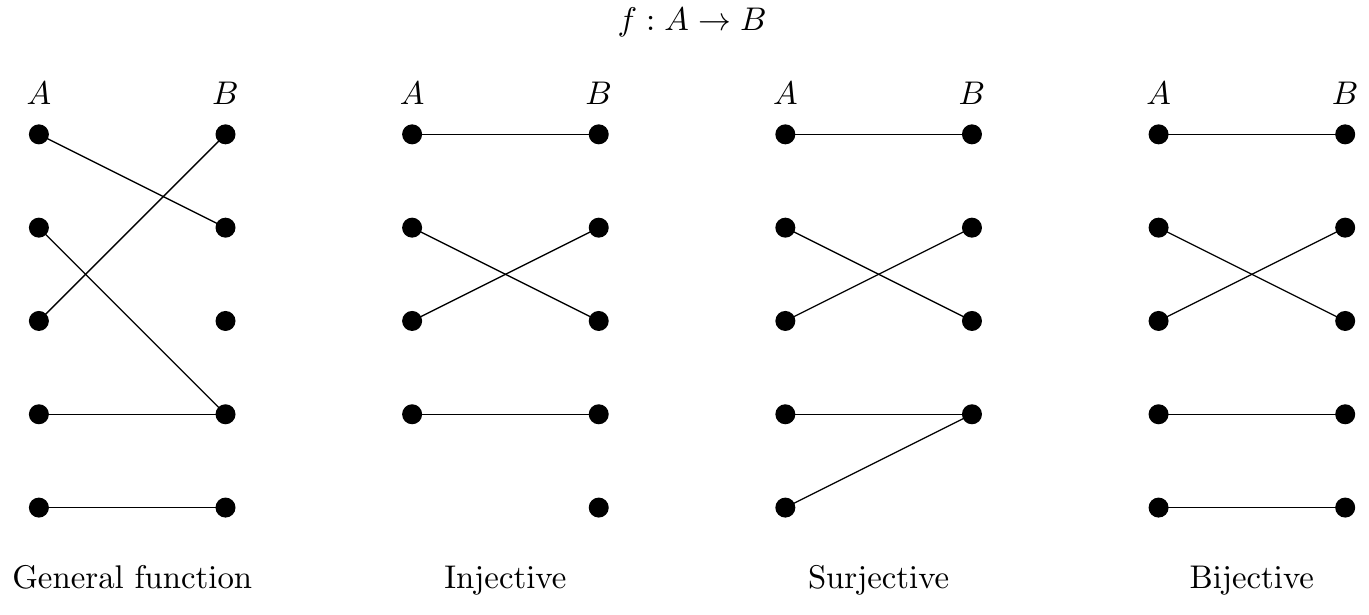
\includegraphics[scale=0.25]{Functions}
\end{center}

\subsubsection*{Example 23.4}

Let \(f:\bb N\to\bb N\) be \(f(x)=x^2\)

\paragraph{Claim} \(f\) is injective

\paragraph{Proof} Let \(x,y\in\bb N\). SUppose \(f(x)=f(y)\), we need to show \(x=y\).
\begin{align*}
f(x)&=f(y)\\
x^2&=y^2\\
x^2-y^2&=0\\
(x-y)(x+y)&=0\\
\end{align*}
\[x-y=0\text{ or }x+y=0\]
\[x+y>0\,\A x,y\in\bb N\]
\[\therefore x-y=0\implies x=y\]
Since \(f(x)=f(y)\implies x=y\) by definition \(f\) is injective. \(\blacksquare\)

\paragraph{Claim} \(f\) is not surjective

\paragraph{Proof} We need to show the negation of surjectivity. That is \(\E y\in\bb N\) such that \(\A x\in\bb N f(x)\ne y\).

If \(y=2\) then \(x^2\ne 2\,\A x\in\bb N\) since \(\sqrt 2\not\in\bb N\). Hence \(f\) is not surjective. \(\blacksquare\)

\begin{example}
Let \(f:\bb Z_{10}\to\bb Z_{10}\) be \(f(\bar x)=2\bar x\)

\paragraph{Claim} \(f\) isn't injective

\paragraph{Proof} We need to show the negation of surjectinity. That is \(\E\bar x,\bar y\in\bb Z_{10}\) such that \(f(\bar x)=f(\bar y)\) but \(\bar x\ne\bar y\)
\[f(\bar 0)=2\cdot\bar 0=\bar 0\]
\[f(\bar 5)=2\cdot\bar 5=\bar 0\text{ since }2\cdot5=10\equiv0\mod10\]
Hence \(f(\bar0)=f(\bar5)\) but \(\bar0\ne\bar5\) so \(f\) is not injective. \(\blacksquare\)

\paragraph{Claim} \(f\) isn't surjective

\paragraph{Proof} We need to show \(\E \bar y\in\bb Z_{10}\) such that \(f(\bar x)=2\bar x\ne\bar y\A x\)
\begin{align*}
\E\bar x\text{ such that }2\bar x=\bar y&\iff\E x\text{ such that }2x\equiv y\mod10\\
&\iff\hcf(2,10)|y\\
&\iff2|y\\
&\implies 2\bar x=\bar 3\text{ has no solutions}
\end{align*}
So \(f\) isn't surjective. \(\blacksquare\)
\end{example}
\begin{example}
Let \(f:\bb Z_{10}\to\bb Z_{10}\) be \(f(\bar x)=3\bar x\)

\paragraph{Claim} \(f\) is bijective

\paragraph{Proof} We need to show that \(f\) is injective and surjective:

\emph{Injectivity:}

Suppose \(f(\bar x)=f(\bar y)\)
\begin{align*}
\implies&3\bar x=3\bar y\\
\implies&3x\equiv3y\mod10\\
\implies&10|3x-3y\\
\implies&10|3(x-y)\\
\implies&10|x-y\\
\implies&x\equiv y\mod10\\
\implies&\bar x=\bar y
\end{align*}
So \(f\) is injective

\emph{Surjectivity}

Let \(\bar y\in\bb Z\)

Then \(f(\bar x=3\bar x\) has a solution \(\iff3x\equiv y\mod10\iff\hcf(3,10)|y\iff 1|y\) which is true \(\A y\). Therefore this always has a solution so \(f\) is surjective.

\(f\) is infective and surjective so \(f\) is bijective. \(\blacksquare\)
\end{example}

\section{Inverse Functions}

If \(f:X\to Y\) is bijective then the inverse of \(f\), denoted \(f^{-1}:Y\to X\) is the function such that
\[f^{-1}(y)=x\iff f(x)=y\]
If \(f:X\to Y\) is bijective then you can solve for \(f^{-1}(y)\) by solving\(f(x)=y\) for \(x\) and setting \(f^{-1}(y)=x\). This definition of inverses gives rise to the following
\[f^{-1}(f(x))=x\,\A x\in X\text{ and }f(f^{-1}(y))=y\,\A y\in Y\]

Let \(f:\bb Z\to\bb Z\) be \(f(n)=n+1\). This is bijective so has an inverse \(f^{-1}(x)=x-1\).

Let \(g:\bb N\to\bb N\) be \(f(n)=n+1\). This is not bijective so has no inverse.

\subsection*{Function Composition}

Let \(S,T,U\) be sets, and let \(f:S\to T\) and \(g:T\to U\) be functions. The composition of \(f\) and \(g\) is the function \(f\circ g:S\to U\) which is defined by the rule
\[(g\circ f)(s)=g(f(s))\,\A s\in S\]

\begin{example}
\paragraph{Claim} If \(f:S\to T\) and \(g:T\to R\) are bijective then \((g\circ f)^{-1}=f^{-1}\circ g^{-1}\)

\paragraph{Proof} We need to verify \(f^{-1}\circ g^{-1}(r)=s\iff r=g\circ f(s)\) for \(s\in S\) and \(r\in R\).
\begin{align*}
f^{-1}\circ g^{-1}(r)=s&\iff f^{-1}(g^{-1}(r))=s\\
\iff& f(f^{-1}(g^{-1}(r)))=f(s)\text{ since \(f\) is injective}\\
\iff& g^{-1}(r)=f(s)\\
\iff& g(g^{-1}(r))=g(f(s))\text{ since \(g\) is injective}\\
\iff& r=g(f(s))=g\circ f(s)\\
\implies& (g\circ f)^{-1}=f^{-1}\circ g^{-1}\quad\blacksquare
\end{align*}
\end{example}

If \(f:X\to Y\) and \(A\subseteq X\) the image of \(A\) under \(f\) is
\[f(A)=\{f(x)|x\in A\}\subseteq Y\]
If \(B\subseteq Y\) the preimage of \(B\) under \(f\) is
\[f^{-1}(B)=\{x\in X|f(x)\in B\}\subseteq X\]
Note that \(f\) does not have to be bijective for this.

\paragraph{Claim} If \(f:X\to Y\) then \(f\) is injective \(\iff f^{-1}(f(A))=A\,\A\subseteq X\)

\paragraph{Proof} Suppose \(f^{-1}(f(A))=A\,\A A\subseteq X\)

Suppose \(f(x)=f(y)=z\). Then \(f^{-1}(f(\{x\}))=\{x\}\) by assumption.
\[f^{-1}(f(\{x\}))=\{a\in \{x\}|f(a)\in f(\{x\})\}=\{z\}\ni y\implies y\in\{x\}\implies y=x\]
Hence \(f\) is injective

Suppose \(f\) is injective. Let \(A\subseteq X\). We want to show \(f^{-1}(f(A))=A\).
\[f^{-1}(f(A))=\{x\in X|f(x)\in f(a)\}\supseteq A\]
So now we need to show \(f^{-1}(f(A))\subseteq A\). Suppose \(\E x\in f^{-1}(f(A))\backslash A\)
\begin{align*}
x\in f^{-1}(f(A))\implies &f(x)\in f(A)=\{f(y)|y\in A\}\\
\implies &\E y\in A\text{ such that }f(y)=f(x)\\
\implies &y=x\text{ since \(f\) is injective}
\end{align*}
However \(x\not\in A\) and \(y\in A\), therefore \(x\ne y\). This is a contradiction, therefore \(f^{-1}(f(A))\subseteq A\) and \(A\subseteq f^{-1}(f(A))\) This can only be true if \(f^{-1}(f(A))=A\). \(\blacksquare\)

Likewise \(f^{-1}(f(B))=B\iff f\) is surjective

It isn't always the case that \(A_1\cap A_2=\emptyset\implies f(A_1)\cap f(A_2)=\emptyset\). If \(f\) isn't injective then it fails. This is because \(\E f(x)=f(y)\) such that \(x\ne y\). Hence \(\{x\}\cap\{y\}=\emptyset\) but \(f(\{x\})\cap f(\{y\})=\{f(x)\}\cap \{f(y)\}=\{f(x)\}\cap \{f(x)\}=\{f(x)\}\ne\emptyset\)

\paragraph{Claim} If \(B_1\cap B_2=\emptyset\) then \(f^{-1}(B_1)\cap f^{-1}(B_2)=\emptyset\)

\paragraph{Proof} We will prove the contrapositive that if \(f^{-1}(B_1)\cap f^{-1}(B_2)\ne\emptyset\) then \(B_1\cap B_2\ne\emptyset\)
\begin{align*}
\E x\in f^{-1}(B_1)\cap f^{-1}(B_2)&\implies\left\{
\begin{array}{l}
x\in f^{-1}(B_1)\implies f(x)\in B_1\\
x\in f^{-1}(B_2)\implies f(x)\in B_2
\end{array}
\right.\\
&\implies f(x)\in B_1\cap B_2\ne\emptyset\quad\blacksquare
\end{align*}

For two sets \(A,B\) \(f^{-1}(A\cap B)=f^{-1}(A)\cap f^{-1}(B)\)

\section{Permutations}

Let \(S_n\) be the set of bijections \(f:\{1,2,\dotsc,n\}\to\{1,2,\dotsc,n\}\). That is the set of all permutations of \(\{1,2,\dotsc,n\}\).

We often denote a permutation \(f\) as
\[f=
\begin{pmatrix}
1 & 2 & \cdots & n\\
f(1) & f(2) & \cdots & f(n)
\end{pmatrix}
\]
When composing two functions \(f\) and \(g\) we often write \(fg=f\circ g\) for convenience. Similarly if we compose \(f\) with itself we write \(f^2=ff=f\circ f\)
\begin{example}
If \(f\) is defined as below what is \(f^2\)?
\[f=
\begin{pmatrix}
1 & 2 & 3 & 4\\
2 & 1 & 4 & 3
\end{pmatrix}
\]
It is often useful to use a table of all elements of \(\{1,2,\dotsc,n\}\) as columns and each row being the result of a permutation:
\[
\begin{array}{c|cccc}
f^2 & 1 & 2 & 3 & 4\\\hline
f & 2 & 1 & 4 & 3\\
f & 1 & 2 & 3 & 4
\end{array}
\implies f^2=
\begin{pmatrix}
1 & 2 & 3 & 4\\
1 & 2 & 3 & 4
\end{pmatrix}
\]
\end{example}
The identity permutation is denoted \(\iota\) and defined as \(f\iota=\iota f=f\). In example 25.1 \(f^2\) is the identity element. This means that \(\iota\in S_n\) and has the property that \(\iota(x)=x\,\A x\).

\(S_n\) forms a group under function composition \((S_n,\circ)\). This means that the four group properties hold:
\begin{itemize}
\item Closure: \(f,g\in S_n\implies fg\in S_n\)
\item Identity: There exists a unique element \(\iota\) such that \(f\in S_n\implies f\iota=\iota f=f\)
\item Inverse: For each \(f\in S_n\) there exists a unique element \(f^{-1}\) such that \(ff^{-1}=f^{-1}f=\iota\)
\item Associativity: For \(f,g,h\in S_n\) \(f(gh)=(fg)h\)
\end{itemize}
To find the inverse \(f^{-1}\) of \(f\) just swap the two rows and then rearrange the columns such that the top row is in order.
\begin{example}
Find the inverse of \(f\) where 
\[f=
\begin{pmatrix}
1 & 2 & 3 & 4 & 5\\
5 & 4 & 1 & 2 & 3
\end{pmatrix}
\]
\[f^{-1}=
\begin{pmatrix}
5 & 4 & 1 & 2 & 3\\
1 & 2 & 3 & 4 & 5
\end{pmatrix}
=
\begin{pmatrix}
1 & 2 & 3 & 4 & 5\\
3 & 4 & 5 & 2 & 1
\end{pmatrix}
\]
\end{example}
Suppose \(f:X\to Y\) and \(g:Y\to X\) and \(gf(x)=x\,\A x\in X\centernot\implies g=f^{-1}\). We also need to show that \(fg(y)=y\,\A y\in Y\) as well before we can say \(g=f^{-1}\). This only works if \(gf\) is a bijection. By closure we know that \(gf\in S_n\) so we know that \(gf\) is a bjection for \(f,g\in S_n\).

It is easy to show that for a non-bijection this property doesn't hold. Let \(f:\{1\}\to \{1,2\}\) and \(g:\{1,2\}\to \{1\}\) be functions defined as \(f(1)=2\) and \(g(1)=g(2)=1\).
\[gf(1)=g(f(1))=g(2)=1\implies gf(x)=x\,\A x\in\{1\}\]
however \(g\ne f^{-1}\) since \(f\) isn't a bijection so doesn't have an inverse.

\paragraph{Claim} If \(f,g\in S_n\) and \(gf=\iota\) then \(g=f^{-1}\)

\paragraph{Proof} By definition fo an inverse:
\begin{align*}
g=f^{-1}\iff&(g(y)=x\iff y=f(x))\\
y=f(x)\iff&g(y)=g(f(x))\\
\iff&g(y)=x\quad\blacksquare
\end{align*}
Because this is true for \(f,g\in S_n\) we can check if \(g=f^{-1}\) by checking that \(gf=\iota\).
\begin{example}
Verify that, for \(f,g\in S_n)\), \((fg)^{-1}=g^{-1}f^{-1}\).

If this is true the \(g^{-1}f^{-1}fg=\iota\)
\[g^{-1}f^{-1}fg=g^{-1}\iota g=g^{-1}g=\iota\]
so \((fg)^{-1}=g^{-1}f^{-1}\)
\end{example}
There is one way in which \(S_n\) is not nicely multiplicative, it is not commutative. This means that \(fg=h\centernot\implies gf=h\).
\begin{example}
\[f=
\begin{pmatrix}
1 & 2 & 3 & 4 & 5\\
3 & 2 & 4 & 5 & 1
\end{pmatrix}
,\qquad g=
\begin{pmatrix}
1 & 2 & 3 & 4 & 5\\
2 & 1 & 3 & 5 & 4
\end{pmatrix}
\]
\[
\begin{array}{c|ccccc}
fg & 1 & 2 & 3 & 4 & 5\\\hline
g & 2 & 1 & 3 & 5 & 4\\
f & 2 & 3 & 4 & 1 & 5
\end{array}
\implies fg
\begin{pmatrix}
1 & 2 & 3 & 4 & 5\\
2 & 3 & 4 & 1 & 5
\end{pmatrix}
\]
\[
\begin{array}{c|ccccc}
gf & 1 & 2 & 3 & 4 & 5\\\hline
f & 3 & 2 & 4 & 5 & 1\\
g & 3 & 1 & 5 & 4 & 2
\end{array}
\implies gf
\begin{pmatrix}
1 & 2 & 3 & 4 & 5\\
3 & 1 & 5 & 4 & 2
\end{pmatrix}
\]
It can be seen that \(fg\ne gf\)
\end{example}

\subsection*{Cycles}

An \(r\)-cycle in \(S_n\) is a permutation of \(f\) such that for some distinct \(a_1,a_2,\dotsc,a_r\) such that \(a_1\xrightarrow{f}a_2\xrightarrow{f}\dotsb\xrightarrow{f}a_{r-1}\xrightarrow{f}a_r\xrightarrow{f}a_1\) and \(f(x)=x\,\A x\not\in\{a_1,a_2,\dotsc,a_r\}\).

We can denote a cycle as above as \((a_1\,a_2\,\dotsc\,a_r)\).
\begin{example}
What cycles are in \(f\) when \(f\) is defined as below?
\[f=
\begin{pmatrix}
1 & 2 & 3 & 4 & 5\\
3 & 2 & 4 & 5 & 1
\end{pmatrix}
\]
\[1\xrightarrow{f}3\xrightarrow{f}4\xrightarrow{f}5\xrightarrow{f}1,\qquad 2\xrightarrow{f}2\]
So \(f\) contains the cycles \((1\,3\,4\,5)\) and \((2)\). We can write \(f\) as a product of these cycles \(f=(1\,3\,4\,5)(2)\). Note that since \((2)\implies f(x)=x\,\A x\) then \((2)=\iota\) since it doesn't change anything. Any 1-cycle is the identity. So we can write \(f=(1\,3\,4\,5)\) and it means the same thing.
\end{example}
\begin{example}
How many possible 5-cycles are there of \(\{1,2,3,4,5\}\)?

Let \(f\) be a 5-cycle \((b_1\,b_2\,\dotsc\,b_5)=(b_2\,b_3\dotsc b_5\,b_1)\). By repeatedly applying this all \(f\) can be written as \((1\, b_1\,\dotsc\, b_4)\). This means that there are 4 choices for \(b_1\), which leaves 3 choices for \(b_2\) etc. By the multiplication principal there are \(4\cdot 3\cdot 2\cdot 1=4!=24\) options so there are 24 5-cylces of \(\{1,2,3,4,5\}\)
\end{example}
In general there are \((n-1)!\) different \(n\)-cycles of \(\{1,2,\dotsc,n\}\).

\section{Cycle decompositions}

To find the inverse of a cycle we invert the cycle
\[(a_1\,a_2\,\dotsc\, a_r)^{-1}=(a_r\, a_r-1\,\dotsc\,a_1)\]

If \(a=(a_1\,a_2\,\dotsc\,a_r)\) and \(b=(b_1\,b_2\,\dotsc\,b_s)\) are disjoint cycles (that is \(a_i\ne b_j\A i,j\)) then the composition of both is commutative
\[a\circ b=b\circ a\]

\subsection*{Cycle decompositions}

Proposition 20.3 proves that all \(f\in S_n\) can be decomposed into disjoint cycles, that is \(f=\alpha_1\alpha_2\dotsm\alpha_k\) where \(\alpha_i\) is disjoint from \(\alpha_j\) if \(i\ne j\).

Given a permutation \(f\) how do we work out the cycle decomposition?

We start with a number \(x\) and look at \(x,f(x),f^2(x)\dotsc\) until we get \(f^k(x)=x\) and this gives us the first cycle \((x\,f(x)\,\dotsc\,f^k(x))\). We then repeat with a number not in this cycle until there are no numbers left not in a cycle.

\begin{example}
What is the cycle decomposition of \(f=(1\,2\,3)(2\,3\,4)(5\,2\,1)\)?

\[
\begin{array}{c|ccccc}
f & 1 & 2 & 3 & 4 & 5\\\hline
(5\,2\,1) & 5 & 1 & 3 & 4 & 2\\
(2\,3\,4) & 5 & 1 & 4 & 2 & 3\\
(1\,2\,3) & 5 & 2 & 4 & 3 & 1
\end{array}
\implies f=
\begin{pmatrix}
1 & 2 & 3 & 4 & 5\\
5 & 2 & 4 & 3 & 1
\end{pmatrix}
\]
\[
\begin{array}{ccc}
1\to 5\to 1 & \implies & (1\,5)\\
2\to 2 & \implies & (2)\\
3\to 4\to 3 & \implies & (3\,4)
\end{array}
\]
\[\implies f=(1\,5)(3\,4)\]
\end{example}
The order of \(f\in S_n\) is the smallest value of \(k\) such that \(f^k=\iota\).

Proposition 20.4 proves that if \(f=\alpha_1\dotsm\alpha_l\) where \(\alpha_i\) are disjoint cycles then the order of \(f\) is the least common multiple of the lengths of the cycles.
\begin{example} 
What is the order of the following permutations?
\begin{enumerate}
\renewcommand{\labelenumi}{(\alph{enumi})}
\item \(f=(1\,2)(\,3\,4\,5)\)
\item \(g=(1\,4\,2)(2\,3\,5)\)
\end{enumerate}~\\[-2em]
\begin{enumerate}
\renewcommand{\labelenumi}{(\alph{enumi})}
\item The order of \(f\) is \(\lcm(2,3)=6\)
\item
\[
\begin{array}{c|ccccc}
f & 1 & 2 & 3 & 4 & 5\\\hline
(1\,4\,2) & 4 & 1 & 3 & 2 & 5\\
(2\,3\,5) & 4 & 1 & 5 & 3 & 2
\end{array}
\implies f=(1\,4\,2\,3\,5)\implies\text{order of \(f\) is }5\]
\end{enumerate}
\end{example}

\section{Sign function}

\begin{example}
Suppose I shuffle 16 cards according to the permutation
\[f=\left(
\begin{pmatrix}
1 & 2 & 3 & 4 & 5 & 6 & 7 & 8 & 9 & 10 & 11 & 12 & 13 & 14 & 15 & 16\\
1 & 9 & 2 & 10 & 3 & 11 & 4 & 12 & 5 & 13 & 6 & 14 & 7 & 15 & 8 & 16
\end{pmatrix}
\right)
\]
How many times do I have to do this to get back to the original order?

This is the same as asking what the order of the \(f\) is.
\[
\begin{array}{cccccc}
1\to 1 & 2\to 9\to 5\to 3\to 2 & 4\to 10\to 13\to 7\to 4 & 6\to 11\to 6 & 8\to 12\to 14\to 15\to 8 &16\to 16\\
(1) & (2\,9\,5\,3) & (4\,10\,13\,7) & (6\,11) & (8\,12\,14\,15) & (16)
\end{array}
\]
\[f= (2\,9\,5\,3)(4\,10\,13\,7)(6\,11)(8\,12\,14\,15)\]
These are cycles of length 2 or 4 so the number of shuffles needed is \(\lcm(2,4)=4\).
\end{example}
\begin{example}
How many permutations of order 6 are there in \(S_5\)?

The only way \(f\in S_5\) can have order 6 is if it is a 2-cylce and a 3-cycle. There are \(\binom 53=10\) different ways to select 3 elements from a set of 5, to form a 3-cycle, and the other two elements can form a 2-cycle. This gives 10 different arrangements of elements into each cycle. Each cycle then has \((3-1)!=2\) or \((2-1)!=1\) possible arrangement. Therefore by the multiplicative principal there are \(10\cdot 2\cdot 1=20\) different cycles of order 6 in \(S_5\).
\end{example}

\subsection*{Sign function}

The sign function \(\sgn\) is a function \(\sgn:S_n\to\{\pm1\}\) such that for \(f,g,\iota\in S_n\) where \(\iota\) is the identity permutation
\begin{itemize}
\item \(\sgn(f)=(-1)^{r-1}\) if \(f\) is an \(r\)-cycle
\item \(\sgn(\iota)=1\)
\item \(\sgn(fg)=\sgn(f)\sgn(g)\)
\item \(\sgn(f^{-1})=\sgn(f)\)
\end{itemize}

\begin{example}
What is the sign of \(f\) where
\[f=
\begin{pmatrix}
1 & 2 & 3 & 4 & 5 & 6 & 7 & 8 & 9 & 10 & 11\\
2 & 3 & 4 & 1 & 6 & 7 & 8 & 9 & 5 & 11 & 10
\end{pmatrix}
\]
\[
\begin{array}{cccccccccc}
1 \to 2 \to 3 \to 4 \to 1 & 5 \to 6 \to 7 \to 8 \to 9 \to 5 & 10 \to 11 \to 10\\
(1\,2\,3\,4) & (5\,6\,7\,8\,9) & (10\,11)
\end{array}
\]
So \(f=(1\,2\,3\,4)(5\,6\,7\,8\,9)(10\,11)\). This means that \(\sgn(f)\) is given by:
\begin{align*}
\sgn(f)&=\sgn((1\,2\,3\,4)(5\,6\,7\,8\,9)(10\,11))\\
&=\sgn(1\,2\,3\,4)\sgn(5\,6\,7\,8\,9)\sgn(10\,11)\\
&=(-1)^{4-1}(-1)^{5-1}(-1^{2-1}\\
&=(-1)^3(-1)^4(-1)^1\\
&=(-1)(1)(-1)\\
&=1
\end{align*}
\end{example}

If \(\sgn(f)=1\) we say \(f\) is even. If \(\sgn(f)=-1\) we say \(f\) is odd.

We say \(S\subseteq S_n\) generates \(S_n\) if every \(f\in S_n\) can be written as a product of functions in \(S\), that is for \(f\in S_n\) \(f=\alpha_1\dotsm\alpha_k\) where \(\alpha_i\in S\).
\begin{example}
\[f=
\begin{pmatrix}
1 & 2 & 3 & 4 & 5\\
2 & 3 & 1 & 5 & 4
\end{pmatrix}\] 
Can \(f\) be written as a product of 2-cycles or a product of 3-cycles?

By proposition 20.6 all permutations can be written as a product of 2-cycles. \(f=(1\,2\,3)(4\,5)\implies\sgn(f)=-1\). If \(\alpha\) is a 3-cycle then \(\sgn(\alpha)=1\) so \(\prod_i\alpha_i\ne-1\) for any \(\alpha,i\), hence there is no way to write \(f\) as a product of 3-cycles.
\end{example}

\section{Infinity}

How do we compare the size of infinite sets?

If \(S\) and \(T\) are finite then \(|S|=|T|\iff f:S\to T\) is a bijection. If \(|S|=n\) then we can list the elements of \(S\) as \(\{s_1,s_2,\dotsc,s_n\}\) so \(f:\{1,2,\dotsc,n\}\to S\) is a bijection and \(f(i)=s_i\). We use this same idea as a motivation for comparing the size of infinite sets.

If \(A\) and \(B\) are sets we say they have the same cardinality if \(\E f:A\to B\) which is a bijection. We write \(|A|=|B|\) or \(A\sim B\).

If \(A\sim\bb N\) we say \(A\) is countable. If \(A\) is infinite and \(A\not\sim\bb N\) we say \(A\) is uncountable.

\paragraph{Claim} If \(S\) is countable and \(T\) is finite then \(S\backslash T\) is countable

\paragraph{Proof} Let us assume \(S\backslash T\) is finite

We can write \(S=(S\backslash T)\cup T\). This means that \(S\) is the union of two finite sets which means \(S\) is finite. This is a contradiction so \(S\backslash T\) must be infinite. By proposition 21.2 every infinite subset of \(\bb N\) is countable. If \(S\) is countable there is a bijection \(f:S\to\bb N\implies f(A)\subseteq\bb N\) where \(f(A)\) is an infinite set. This means \(A\sim f(A)\sim\bb N\). \(\sim\) is an equivalence relation so \(A\sim \bb N\) which means that \(A\) is countable if it is an infinite subset of \(S\). This means that \(S\backslash T\) is countable. \(\blacksquare\)

If \(S\) and \(T\subseteq S\) are both countable we can't conclude anything about the size of \(S\backslash T\)
\begin{itemize}
\item Let \(S=\bb N\) and \(T=2n\) where \(n\in\bb N\). This means that \(T\) is the set of even numbers so \(S\backslash T\) is the set of odd numbers. This is an infinite subset of \(\bb N\) so \(S\backslash T\) is countable

\item Let \(S=T\) then \(S\backslash T=\emptyset\) is empty

\item Let \(T=S\backslash s_1\) this means \(S\backslash T=s_1\) has finite size
\end{itemize}
So \(S\backslash T\) can be countable, finite or empty

\begin{example}
Let \(f:S\to\bb N\) and \(g:\bb N\to S\) be functions where \(S\) is infinite. Which of the following properties imply that \(S\) is countable?
\begin{itemize}
\item \(f\) is injective -- By proposition 21.4 (the injection lemma) if \(S\) is infinite and \(f:S\to \bb N\) is injective then \(S\sim\bb N\).

\item \(f\) is surjective -- This doesn't mean that \(S\) is countable. A counter example is \(f:\bb R_+\to\bb N\) and \(f(x)=\lfloor x\rfloor\) is surjective but \(\bb R_+\) is uncountable.

\item \(g\) is injective -- This doesn't mean that \(S\) is countable. A counter example is \(g:\bb N\to\bb R\) and \(g(n)=n\) is injective byt \(\bb R\) is uncountable.

\item \(g\) is surjective -- This does mean that \(S\) is countable by the surjection lemma
\end{itemize}
\end{example}

\subsubsection*{Surjection Lemma}

\paragraph{Claim} If \(g:\bb N\to S\) is surjective and \(S\) is infinite then \(S\) is countable.

\paragraph{Proof} We need to show that there is an injective function \(h:S\to\bb N\) then by the injective lemma \(S\sim\bb N\) so \(S\) is countable.

Since \(g\) is surjective \(\implies\A x\in S\E y\in\bb N\) such that \(g(y)=x\)

Set \(h(x)=y\implies g(h(x))=g(y)=x\)

Suppose \(h(x)=h(y)\) we need to show that this means \(x=y\) so \(h\) is injective

By our coice of \(h\) we know \(g(h(x))=x\implies g(h(y))=x\implies x=y\) so \(h\) is injective so by the injection lemma \(S\) is countable. \(\blacksquare\)

\subsubsection*{Better Injection Lemma}

\paragraph{Claim} If \(A\) is infinite and \(B\) is countable and there is an injection \(f:A\to B\) then \(A\) is countable.

\paragraph{Proof} Since \(B\sim\bb N\E g:B\to\bb N\) which is a bijection \(\implies g\circ f:A\to\bb N\) is injective so by the injection lemma \(A\sim\bb N\). \(\blacksquare\)

\begin{example}
\paragraph{Claim} \(\bb N\times\bb N\) is countable

\paragraph{Proof} We need to show that there exists \(f:\bb N\times\bb N\to\bb N\).

One such function is \(f(m,n)=2^m3^n\). Since prime factorisations are unique this is injective. Also \(\bb N\times\bb N\) is infinite as there are a countably infinite number of options for \(n\) in \((1,n)\). So \(\bb N\times\bb N\) is infinite and there is an injection to \(\bb N\). This means that \(\bb N\times \bb N\sim \bb N\). \(\blacksquare\)

This example extends using \(n\) distinct primes for \(\bb N^n\)
\end{example}
\begin{example}
\paragraph{Claim} \(\bb Q\sim\bb N\)

\paragraph{Proof} We can write every element in \(\bb Q\) uniquely as \(\frac mn\) where \(m,n\in\bb Z\), \(n>0\) and \(\hcf(m,n)=1\). This means that there is an injection \(f:\left(\frac mn\right)\to (m,n)\in\bb N\times\bb N\) so by the better injection lemma \(\bb Q\sim \bb N\times\bb N\implies \bb Q\sim \bb N\). \(\blacksquare\)
\end{example}


\section{Larger infinities}

How big can a collection \(\mathcal{C}\) of non-overlapping (disjoint) squares in \(\bb R^2\) be?

\paragraph{Claim} If \(\mathcal{C}\) is infinite then it is countable

\paragraph{Proof} Let \(c\in\mathcal C\)

\begin{center}
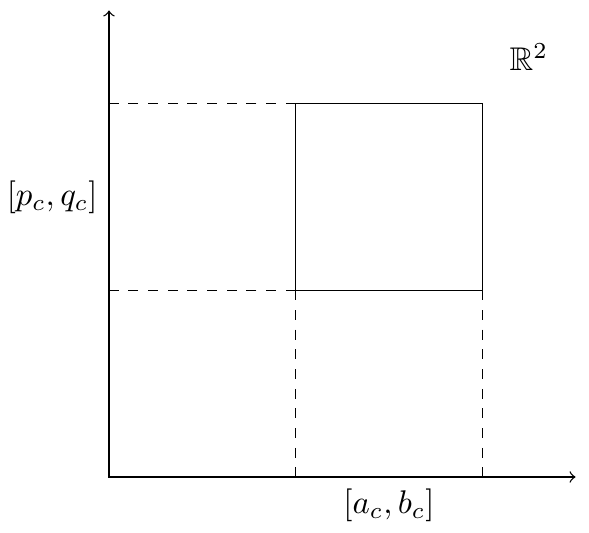
\includegraphics[scale=0.3]{SquaresInR2}
\end{center}

\(\A c\E a_c,b_c,p_c,q_c\in\bb R\) such that \(c=[a_c,b_c]\times[p_c,q_c]\)

We know \(\E r_c\in[a_c,b_c]\cap\bb Q\) and \(\E s_c\in[p_c,q_c]\cap\bb Q\)

Let \(f:\mathcal C\to \bb Q^2\) be \(f(c)=(r_c,s_c)\)

\(f\) is injective since if \(c\) and \(c'\) are distinct squares then \(c\cap c=\emptyset\)

So \(f(c)\in c\implies f(c')\not\in c'\implies f(c)\ne f(c')\)

By the better injection lemman since \(\bb Q^2\) is countable and \(f:\mathcal C\to \bb Q^2\) is injective \(\mathcal C\) is countable. \(\blacksquare\)

\paragraph{Claim} If \(S\) is uncountable and \(T\) is countable then \(S\backslash T\) is uncountable.

\paragraph{Lemma} If \(A\sim\bb N\sim B\) then \(A\cup B\sim\bb N\)

\paragraph{Proof} \(A\sim\bb N\implies\E\) a bijection \(f:A\to\bb N\)

\(B\sim\bb N\implies\E\) a bijection \(g:B\to\bb N\)

Define \(h:A\cup B\to\bb N^2\) as
\[h(x)=\left\{
\begin{array}{cc}
(f(x),1) & \text{if }x\in A\\
(g(x),2) & \text{if }x\in B\backslash A
\end{array}
\right.\]
We need to show that \(h\) is injective and then by the better injection lemma \(A\cup B\sim\bb N\).

Suppose \(h(x)=h(y)\implies\) the right coordinates are the same. This means either \(x,y\in A\) or \(x,y\in B\backslash A\).
\emph{Case 1:} \(x,y\in A\)
\[\implies h(x)=(f(x),1)=(f(y),1)=h(y)\implies f(x)=f(y)\implies x=y\]
since \(f\) is bijective.

\emph{Case 2:} \(x,y\in B\backslash A\)
\[\implies h(x)=(g(x),2)=(g(y),2)=h(y)\implies g(x)=g(y)\implies x=y\]
since \(g\) is bijective.

\(h\) is injective in all cases so \(h\) is injective. Therefore by the better injection lemma \(A\cup B\sim\bb N\). 

Since \(S=(S\backslash T)\cup T\) if \(S\backslash T\) is countable then \(S\) is countable. This is a contradiction so \(S\backslash T\) must be uncountable. \(\blacksquare\)

The power set of a set \(S\) is denoted \(\mathcal P(S)\) and is the set of all subsets of \(S\) including \(\emptyset\) and \(S\).
\[\mathcal P(S)=\{A|A\subseteq S\}\]
The size of \(\mathcal P(S)\) is \(2^{|S|}\). If \(S\) is infinite then \(|\mathcal P(S)|\) is a larger infinity by proposition 21.5. This means that repeatedly taking the power set results in an infinite number of different sized infinities, if \(S\) is countable then
\[|\bb N|\sim|S|<|\mathcal P(S)|<|\mathcal P(\mathcal P(S))|<|\mathcal P(\mathcal P(\mathcal P(S)))|<\dotsb\]

How do we prove a set \(S\) is uncountable?

One way to do this is avoidance. Assume \(S\) is countable and as such can be listed as \(S=\{s_1,s_2,\dotsc\}\) and then construct \(s\in S\) such that \(s\ne s_i\A i\)

\begin{example}
Let \(S=\{(a_1,a_2,\dotsc)|a_i\in \{0,1\}\}\)

\paragraph{Claim} \(|S|>|N|\)

\paragraph{Proof 1} Suppose \(|S|=|\bb N|\), then 
\[S=\{s_1,s_2,\dotsc\}\]
\[s_i=(a_1^i,a_2^i,\dotsc)\text{ where }a_j^i\in\{0,1\}\]

Now define \(s=(b_1,b_2,\dotsc)\) where
\[b_i=\left\{
\begin{array}{cc}
0 & \text{if }a_i^i=1\\
1 & \text{if }a_i^i=0
\end{array}
\right.\]
This means that \(s\ne s_i\A i\) as if \(\E i\) such that \(s=s_i\) then \(b_i=a_i^i\) and this is a contradiction to the definition of \(s\). This means \(s\not\in\{s_1,s_2,\dotsc\}=S\) this is a contradiction since \(s\in S\) so \(|S|>|\bb N|\). \(\blacksquare\)

Another method is to find a bijection \(f:S\to T\) where \(|T|>|\bb N|\)

\paragraph{Proof 2} Let \(\mathcal P(\bb N)=\{A\subseteq\bb N\}\) and let \(f:\mathcal P(\bb N)\to S\) where \(f(A)=(a_1^A,a_2^A,\dotsc)\) where
\[a_i^A=\left\{
\begin{array}{cc}
1 & \text{if }i\in A\\
0 & \text{if }i\not\in A
\end{array}
\right.\]
Since all \(A\) are unique this means that \(A,B\in\mathcal P(N)\) must have at least one element different and therefore this corresponds to a difference in one of the \(a_i^A\) and \(b_i^B\). This means \(f\) is injective. Since every subset of \(\bb N\) constructs an countably long tuple we must get every possible infinitely long tuple under the constraints. This means \(f:\mathcal P(\bb N)\to S\) is a bijection therefore \(|S|=|\mathcal P(A)|>|\bb N|\). \(\blacksquare\)

A final method is to find an injection from an uncountable set to \(S\)

\paragraph{Proof 3} If there is an injection \(f:A\to S\) then \(|A|\le|S|\implies\) if \(|A|>|\bb N|\) then \(|S|>|\bb N|\). \(\blacksquare\)
\end{example}

\paragraph{Claim} \(|\bb R|=|(0,\infty)|\)

\paragraph{Proof} Construct a bijection \(f:(0,\infty)\to\bb R\)
\[f(x)=x-\frac 1x\]
is a bijection from \((0,\infty)\to \bb R\) hence \(|(0,\infty)|=|\bb R|\). \(\blacksquare\)

\section{Bounds}

A set \(A\subseteq\bb R\) is
\begin{itemize}
\item bounded above if \(\E M\) such that \(\A x\in A x\le M\)
\item bounded below if \(\E m\) such that \(\A x\in A x\ge m\)
\item bounded if it is bounded above and below
\end{itemize}

\begin{example}
\paragraph{Claim} \(S=\{x|x^2-x-2<0\}\) is bounded

\paragraph{Proof} Let \(x\in S\) then \(0>x^2-x-2=(x+1)(x-2)\)

Exactly one of these must be negative and since \(x+1>x-2\) this means
\[x-2<0<x+1\implies -1<x<2\A x\in S\]
so \(S\) is bounded. \(\blacksquare\)
\end{example}
\begin{example}
\paragraph{Claim} \(A=\{n+(-1)^nn|n\in\bb N\}\) is bounded below

\paragraph{Proof} If \(n+(-1)^nn\in A\) then \(n+(-1)^nn\ge n-n=0\implies x\ge 0\A x\in A\implies A\) is bounded below. \(\blacksquare\)

\paragraph{Claim} \(A=\{n+(-1)^nn|n\in\bb N\}\) is unbounded below

\paragraph{Proof} We need to show the negation of the condition for bounded above
\[\A M\E x\in A\text{ such that } x>M\]
Let \(M\in\bb R\). We need to show that there exists \(x\in A\) such that \(x>M\)

\emph{Case 1} \(M\le 0\) then \(x\ge 0\ge M\A x\in A\)

\emph{Case 2} Suppose \(M>0\)

We need to find \(n+(-1)^nn>M\)

Let \(n=2m\) then \(n+(-1)^nn=2m+2m=4m\)

Let \(m>\frac{M}{4}\) then \(n+(-1)^nn=4m>M\). \(\blacksquare\)
\end{example}

\subsection*{Least Upper Bound}

If \(A\subseteq\bb R\) is bounded above then the least upper bound of \(A\) \((\LUB(A))\) is the number such that
\begin{itemize}
\item \(\A x\in A x\le\LUB(A)\) (ie \(\LUB(A)\) is an upper bound)
\item If \(y<\LUB(A)\) then \(\E x\in A\) such that \(x>y\) (ie \(y\) is not an upper bound)
\end{itemize}

\begin{example}
\paragraph{Claim} If \(A=\{x\in\bb Q|x<\sqrt 2\}\) then \(\LUB(A)=\sqrt 2\)

\paragraph{Proof} \(x<\sqrt 2\A x\in A\) by definition. This means that \(\sqrt 2\) is an upper bound.

Let \(y<\sqrt 2\). We have previously shown that \(\A a<b\E r\in\bb Q\cap(a,b)\)

This means \(\E x\in\bb Q\cap(y,\sqrt 2)\implies x\in A\) and \(x>y\) hence the upper bound can't be less than \(\sqrt 2\). This means that \(\LUB(A)=\sqrt 2\). \(\blacksquare\)
\end{example}

\begin{example}
\paragraph{Claim} If \(A=\{1-n^{(-1)^n}|n\in\bb N\) then \(\LUB(A)=1\)

\paragraph{Proof} \(1-n^{(-1)^n}<1\A n>0\) therefore 1 is an upper bound.

Let \(y<1\), we need to show \(\E x\in A\) such that \(x>y\)

Let \(n=2m+1\) then \(1-n^{(-1)^n}=1-\frac{1}{2m+1}\)

So  we need to find \(m\) such that
\begin{align*}
1-\frac{1}{2m+1}>y\iff &\frac{1}{2m+1}<1-y\\
\iff &2m+1>\frac{1}{1-y}\\
\iff &m>\left(\frac{1}{1-y}-1\right)/2\\
\end{align*}
Let \(\displaystyle{m=\left\lceil\left(\frac{1}{y-1}-1\right)/2\right\rceil}\)

Then \(A\ni 1-(2m+1)^{(-1)^{2m+1}}>y\) so \(1=\LUB(A)\). \(\blacksquare\)
\end{example}
Which of the following are true?
\begin{enumerate}
\item If \(\alpha>0\) and \(\alpha A=\{\alpha x|x\in A\}\) then \(\LUB(\alpha A)=\alpha\LUB(A)\)
\item If \(-A=\{-x|x\in A\}\) then \(\LUB(-A)=-\LUB(A)\)
\item \(\LUB(A)=\max(A)\)
\item If \(c\in\bb R\) and \(c+A=\{c+x|x\in A\}\) then \(\LUB(c+A)=c+\LUB(A)\)
\end{enumerate}~\\[-2em]
\begin{enumerate}
\item This is true. To show \(\LUB(\alpha A)=\alpha\LUB(A)\) we need to show
\begin{enumerate}
\item \(x\le\alpha\LUB(A)\A x\in\alpha A\)

Let \(x\in\alpha A\implies x=\alpha a\) for some \(a\in A\implies a\le\LUB(A)\implies x=\alpha a\le\alpha\LUB(A)\)
\item \(\A y<\alpha\LUB(A)E x\in\alpha A\) such that \(x>y\)

Let \(y<\alpha\LUB(A)\)
\begin{align*}
\implies &\frac y\alpha<\LUB(A)\\
\implies &\E a\in A\text{ such that }a>\frac y\alpha\\
\implies &y<\frac{\alpha a}{x}\in\alpha A\qquad\blacksquare
\end{align*}
\end{enumerate}
\item This is false. This can be shown by proof by counterexample

Let \(A=(-1,2)\implies\LUB(A)=2\)

\(-A=(-2,1)\implies\LUB(A)=1\ne -2\) as we would expect if \(\LUB(-A)=-\LUB(A)\)

\item This is false. This can be shown by proof by counterexample

For example \(\LUB(0,1)=1\) and \(\max(0,1)\) doesn't exist.

\paragraph{Claim} \(\max(0,1)\) doesn't exist

\paragraph{Proof} Suppose \(m=\max(0,1)\in(0,1)\)

\(\implies m<1\) but as we have shown there is always a rational between any two rationals, in this case \(m<\frac{m+1}{2}\in (0,1)\). This is a contradiction since \(m=\max(0,1)\) so \(\max(0,1)\) doesn't exist. \(\blacksquare\)

\item This is true. To show \(\LUB(c+A)=c+\LUB(A)\) we need to show
\begin{enumerate}
\item \(x\le c+\LUB(A)\A x\in c+A\)

Let \(x\in c+A\implies x=c+a\) for some \(a\in A\implies a\le\LUB(A)\implies x=c+a\le c+\LUB(A)\)

\item \(\A y< c+\LUB(A)\E x\in c+A\) such that \(x>y\)

Let \(y<c+\LUB(A)\)
\begin{align*}
\implies &y-c<\LUB(A)\\
\implies &\E a\in A\text{ such that }a>y-c\\
\implies &y<\frac{a+c}{x}\in A+c\qquad\blacksquare
\end{align*}
\end{enumerate}
\end{enumerate}

\subsection*{Completeness axion}
The completeness axiom states
\begin{displayquote}
Every non-empty set of real numbers with an upper bound must have a least upper bound in \(\bb R\)
\end{displayquote}
\end{document}